\documentclass{article}

% if you need to pass options to natbib, use, e.g.:
% \PassOptionsToPackage{numbers, compress}{natbib}
% before loading nips_2018

% ready for submission
\usepackage{nips_2018}

% to compile a preprint version, e.g., for submission to arXiv, add
% add the [preprint] option:
% \usepackage[preprint]{nips_2018}

% to compile a camera-ready version, add the [final] option, e.g.:
% \usepackage[final]{nips_2018}

% to avoid loading the natbib package, add option nonatbib:
% \usepackage[nonatbib]{nips_2018}

\usepackage[utf8]{inputenc} % allow utf-8 input
\usepackage[T1]{fontenc}    % use 8-bit T1 fonts
\usepackage{hyperref}       % hyperlinks
\usepackage{url}            % simple URL typesetting
\usepackage{booktabs}       % professional-quality tables
\usepackage{amsfonts}       % blackboard math symbols
\usepackage{nicefrac}       % compact symbols for 1/2, etc.
\usepackage{microtype}      % microtypography
\usepackage{amsmath}
\usepackage{amssymb}
\usepackage{amsthm}
\usepackage{bm}
\usepackage{todonotes}
\usepackage{algorithm}
\usepackage{algorithmic}
\usepackage{thmtools, thm-restate}
\usepackage{subcaption}

\newtheorem{lemma}{Lemma}
\newtheorem{theorem}{Theorem}
\newtheorem{corollary}{Corollary}
\newtheorem{remark}{Remark}
\newtheorem{definition}{Definition}
\newtheorem{proposition}{Proposition}

\newcommand{\argmin}{\operatornamewithlimits{argmin}}
\newcommand{\argmax}{\operatornamewithlimits{argmax}}
\newcommand{\arginf}{\operatornamewithlimits{arginf}}
\newcommand{\argsup}{\operatornamewithlimits{argsup}}
\newcommand{\mm}{\operatornamewithlimits{mm}}
\newcommand{\wt}[1]{\widetilde{#1}}
\newcommand{\wh}[1]{\widehat{#1}}
\newcommand{\norm}[1]{\left\lVert #1 \right\rVert}
\newcommand{\abs}[1]{\left\lvert #1 \right\rvert}
\title{Variational Approximations for Transfer in Reinforcement Learning}

% The \author macro works with any number of authors. There are two
% commands used to separate the names and addresses of multiple
% authors: \And and \AND.
%
% Using \And between authors leaves it to LaTeX to determine where to
% break the lines. Using \AND forces a line break at that point. So,
% if LaTeX puts 3 of 4 authors names on the first line, and the last
% on the second line, try using \AND instead of \And before the third
% author name.

\author{
  David S.~Hippocampus\thanks{Use footnote for providing further
    information about author (webpage, alternative
    address)---\emph{not} for acknowledging funding agencies.} \\
  Department of Computer Science\\
  Cranberry-Lemon University\\
  Pittsburgh, PA 15213 \\
  \texttt{hippo@cs.cranberry-lemon.edu} \\
  %% examples of more authors
  %% \And
  %% Coauthor \\
  %% Affiliation \\
  %% Address \\
  %% \texttt{email} \\
  %% \AND
  %% Coauthor \\
  %% Affiliation \\
  %% Address \\
  %% \texttt{email} \\
  %% \And
  %% Coauthor \\
  %% Affiliation \\
  %% Address \\
  %% \texttt{email} \\
  %% \And
  %% Coauthor \\
  %% Affiliation \\
  %% Address \\
  %% \texttt{email} \\
}

\begin{document}
% \nipsfinalcopy is no longer used

\maketitle

\begin{abstract}
  The abstract paragraph should be indented \nicefrac{1}{2}~inch
  (3~picas) on both the left- and right-hand margins. Use 10~point
  type, with a vertical spacing (leading) of 11~points.  The word
  \textbf{Abstract} must be centered, bold, and in point size 12. Two
  line spaces precede the abstract. The abstract must be limited to
  one paragraph.
\end{abstract}

\section{Introduction}

Recent advancements have allowed reinforcement learning (RL) \cite{sutton1998reinforcement} to achieve impressive results in a wide variety of complex tasks, ranging from Atari \cite{mnih2015human}, to the game of Go \cite{silver2016mastering}, to the control of sophisticated robotics systems \cite{kober2009policy,lillicrap2015continuous,levine2016end}. The main limitation is that RL algorithms still require an enormous amount of experience samples before successfully learning such complicated tasks. One of the most promising solutions is transfer learning, which focuses on reusing past knowledge available to the agent in order to reduce the sample-complexity for learning new tasks. In the typical settings of transfer in RL \cite{taylor2009transfer}, the agent is assumed to have already solved a set of \textit{source tasks} generated from some unknown distribution. Then, given a \textit{target task} drawn from the same distribution, or a slightly different one, the agent can rely on knowledge from the source tasks to speed up the learning process. This constitutes a significant advantage over plain RL, where the agent learns each new task from scratch independently of previous learning experience. Several algorithms have been proposed in the literature to transfer experience samples \cite{lazaric2008transfer,taylor2008transferring}, policies/options \cite{fernandez2006probabilistic,konidaris2007building}, rewards \cite{konidaris2006autonomous}, features \cite{barreto2017successor}, parameters \cite{doshi2016hidden,killian2017robust}, and so on. We refer the reader to \cite{taylor2009transfer} for a thorough survey on transfer in RL.

%\paragraph*{Exploration-based introduction}
%One of the most relevant problems in this context is how to efficiently explore the target task based on knowledge from the source tasks. Intuitively, assuming the tasks under consideration share some similarities due to the common distribution, much better exploration strategies than uninformed ones (e.g., $\epsilon$-greedy) can be adopted for quickly learning the target task. Among the appealing approaches for this problem we find Bayesian methods (e.g., \cite{}), which are able to model the uncertainty over the current task based on previous knowledge and drive exploration so that this uncertainty is reduced as quickly as possible. Similarly, model-based algorithms (e.g., \cite{}) typically transfer samples to improve their estimates of the task model and adopt classic count-based exploration to drive the agent towards regions where such estimates are more uncertain. However, all these approaches either require strong assumptions (for example, on the distribution involved in Bayesian methods) or do not scale well to large problems. This greatly limits their practical applicability.

%In this work, we tackle such limitations by considering a more general approach. Similarly to \cite{}, we assume tasks to share similarities in their value functions and use the given source tasks to learn the distribution over such functions. Then, we use this distribution as a prior for learning the target task and we propose and efficient variational approximation of the corresponding posterior. Leveraging on recent ideas from randomized value functions (\cite{}), we design a Thompson sampling-based algorithm which efficiently explores the target task by repeatedly sampling from the posterior and acting greedily w.r.t. (with respect to) the sampled value function. We show that our approach is very general, in the sense that it does not require any specific choice of function approximator or prior/posterior distribution models. \todo[inline]{Maybe mention something about theory/experiments here}

Under the assumption that tasks follow a certain distribution, an intuitive choice for designing a transfer algorithm is to attempt at characterizing the uncertainty over the target task. Then, an ideal algorithm would leverage prior knowledge from the source tasks to interact with the target task in such a way that this uncertainty is reduced as quickly as possible. This simple intuition makes Bayesian \todo{probabilistic? distributional?} methods appealing approaches for transfer in RL, and many previous works have been proposed in this direction. \cite{wilson2007multi} assume tasks share similarities in their dynamics and rewards and propose a hierarchical Bayesian model for the distribution of these two elements. Similarly, \cite{lazaric2010bayesian} assume tasks are similar in their value functions and design a different hierarchical Bayesian model for transferring such information. More recently, \cite{doshi2016hidden}, and its extension \cite{killian2017robust}, consider tasks whose dynamics are governed by some hidden parameters, and propose efficient Bayesian models for quickly learning such parameters in new tasks. However, all these algorithms require specific, and sometimes restrictive, assumptions (e.g., on the distributions involved or the function approximators adopted), which might limit their practical applicability. The importance of having transfer algorithms that alleviate the need of strong assumptions and that can be easily adapted to different contexts motivates us to take a more general approach.

Similarly to \cite{lazaric2010bayesian}, we assume tasks to share similarities in their value functions and use the given source tasks to learn a distribution over such functions. Then, we use this distribution as a prior for learning the target task and we propose and efficient variational approximation of the corresponding posterior. Leveraging on recent ideas from randomized value functions \cite{osband2014generalization}, we design a Thompson Sampling-based algorithm which efficiently explores the target task by repeatedly sampling from the posterior and acting greedily w.r.t. (with respect to) the sampled value function. We show that our approach is very general, in the sense that it does not require any specific choice of function approximator or prior/posterior distribution models. We propose a finite-sample analysis that theoretically validates our approach, while empirically evaluating its performance on three domains with increasing level of difficulty.

\section{Preliminaries}

We consider a distribution $\mathcal{D}$ over tasks, where each task is modeled as a discounted Markov Decision Process (MDP). We define an MDP as a tuple $\mathcal{M} = \langle \mathcal{S},\mathcal{A},\mathcal{P},\mathcal{R},p_0,\gamma\rangle$\todo{Should we provide a more transfer-oriented definition?}, where $\mathcal{S}$ is the state-space, $\mathcal{A}$ is a finite set of actions, $\mathcal{P}(\cdot | s,a)$ is the distribution of the next state $s'$ given that action $a$ is taken in state $s$, $\mathcal{R}: \mathcal{S}\times\mathcal{A}\rightarrow\mathbb{R}$ is the reward function, $p_0$ is the initial-state distribution, and $\gamma\in [0,1)$ is the discount factor. We assume the reward function to be uniformly bounded by a constant $R_{max}>0$. A deterministic policy $\pi : \mathcal{S} \rightarrow \mathcal{A}$ is a mapping from states to actions. At the beginning of each episode of interaction, the initial state $s_0$ is drawn from $p_0$. Then, the agent takes the action $a_0 = \pi(s_0)$, receives a reward $\mathcal{R}(s_0,a_0)$, transitions to the next state $s_1 \sim \mathcal{P}(\cdot | s_0,a_0)$, and the process is repeated. The goal is to find the policy maximizing the long-term return over a possibly infinite horizon: $\max_{\pi}J(\pi)\triangleq\mathbb{E}[\sum_{t=0}^{\infty} \gamma^t r_t \mid \mathcal{M},\pi]$. To this end, we define the optimal value function $Q^*(s,a)$ as the expected return obtained by taking action $a$ in state $s$ and following an optimal policy thereafter. Then, an optimal policy $\pi^*$ is a policy that is greedy with respect to the optimal value function, i.e., $\pi^*(s) = \argmax_a Q^*(s,a)$ for all states $s$. It can be shown (e.g., \cite{puterman1994markov}) that $Q^*$ is the unique fixed-point of the optimal Bellman operator $T$ defined by $TQ(s,a) = \mathcal{R}(s,a) + \gamma\mathbb{E}_{\mathcal{P}}[\max_{a'}Q(s',a')]$ for any value function $Q$. From now on, we adopt the term $Q$-function to denote any plausible value function, i.e., any function $Q : \mathcal{S}\times\mathcal{A} \rightarrow \mathbb{R}$ uniformly bounded by $\frac{R_{max}}{1-\gamma}$.

We consider a parametric family of $Q$-functions, $\mathcal{Q} = \left\{ Q_{\bm{w}} : \mathcal{S}\times\mathcal{A} \rightarrow \mathbb{R} \mid \bm{w}\in\mathbb{R}^K\right\}$, and we assume each function in $\mathcal{Q}$ to be uniformly bounded by $\frac{R_{max}}{1-\gamma}$. When learning the optimal value function, a quantity of interest is how close a given function $Q_{\bm{w}}$ is to the fixed-point of the Bellman operator. A possible measure is its Bellman error (or Bellman residual), defined by $B(\bm{w}) \triangleq TQ_{\bm{w}} - Q_{\bm{w}}$. Notice that $Q_{\bm{w}}$ is optimal if, and only if, $B(\bm{w})(s,a) = 0$ for all $s,a$. If we assume the existence of a distribution $\nu$ over $\mathcal{S}\times\mathcal{A}$, an appealing objective is to directly minimize the squared Bellman error of $Q_{\bm{w}}$ under $\nu$, denoted by $\norm{B(\bm{w})}_{\nu}^2$\todo{Should we define norms before?}. Unfortunately, it is well-known that an unbiased estimator of this quanitity requires two independent samples of the next state $s'$ for each $s,a$ (e.g., \cite{maillard2010finite}). In practice, the Bellman error is typically replaced by the TD error $b(\bm{w})$, which approximates the former using a single transition sample, $b(\bm{w}) = r + \gamma\max_{a'}Q_{\bm{w}}(s',a') - Q_{\bm{w}}(s,a)$. Finally, given a dataset $D = \langle s_i,a_i,r_i,s_i' \rangle_{i=1}^{N}$ of $N$ samples, the squared TD error is computed as $\norm{B(\bm{w})}_{D}^2 = \frac{1}{N}\sum_{i=1}^N (r_i + \gamma \max_{a'} Q_{\bm{w}}(s_i',a') - Q_{\bm{w}}(s_i,a_i))^2 = \frac{1}{N}\sum_{i=1}^N b_i(\bm{w})^2$. Whenever the distinction is clear from the context, with slight abuse of terminology, we refer to the squared Bellman error and squared TD error as Bellman error and TD error, respectively.

%\subsection{Variational Inference}
%
%When working with Bayesian approaches, the posterior distribution of hidden variables $\bm{w} \in \mathbb{R}^K$ given data $D$,
%\begin{equation}\label{eq:bayes}
%p(\bm{w} | D) = \frac{p(D | \bm{w})p(\bm{w})}{p(D)} = \frac{p(D | \bm{w})p(\bm{w})}{\int_{\bm{w}} p(D | \bm{w})p(\bm{w})},
%\end{equation}
%is typically intractable for many models of interest (e.g., when working with deep neural networks) due to difficulties in computing the integral of Eq. \eqref{eq:bayes}. The main intuition behind variational inference \cite{} \todo{CITE} is to approximate the intractable posterior $p(\bm{w} | D)$ with a simpler distribution $q_{\bm{\xi}}(\bm{w})$. The latter is chosen in a parametric family, with variational parameters $\bm{\xi}$, as the minimizer of the Kullback-Leibler (KL) divergence w.r.t. $p$:
%\begin{equation}
%\min_{\bm{\xi}} KL\left(q_{\bm{\xi}}(\bm{w})\ ||\ p(\bm{w} \mid D)\right)
%\end{equation}
%It is well-known that minimizing the KL divergence is equivalent to maximizing the so-called \textit{evidence lower bound} (ELBO), which is defined as:
%\begin{equation}
%\text{ELBO}(\bm{\xi}) = \mathbb{E}_{\bm{w} \sim q_{\bm{\xi}}}\left[ \log p(D | \bm{w}) \right] - KL\left(q_{\bm{\xi}}(\bm{w})\ ||\ p(\bm{w})\right)
%\end{equation}
%Intuitively, the best approximation is the one that maximizes the expected log-likelihood of the data, while minimizing the KL divergenge w.r.t. the prior $p(\bm{w})$.

\section{Variational Transfer Learning}

In this section, we describe our variational approach to transfer in RL. In Section \ref{sec:alg}, we start by introducing our algorithm from a high-level perspective, in such a way that it can be used for any choice of prior and posterior distributions. Then, in Sections \ref{sec:gvt} and \ref{sec:mgvt}, we propose practical implementations based on Gaussians and mixtures of Gaussians, respectively. We conclude with some considerations on how to optimize the proposed objective in Sec. \ref{sec:td}.

\subsection{Algorithm}\label{sec:alg}

We begin with a simple consideration: the distribution $\mathcal{D}$ over tasks clearly induces a distribution over optimal $Q$-functions. \todo{Should we just make the assumption that Q-functions share knowledge in their weights?} Moreover, for any MDP, learning its optimal $Q$-function is sufficient for solving the problem. Thus, one can safely replace the distribution over tasks with the distribution over their optimal value functions. In our parametric settings, we reduce the latter to a distribution $p(\bm{w})$ over weights.
 
Assume, for the moment, that we know the distribution $p(\bm{w})$ and consider a dataset $D=\left\{(s_i,a_i,s_i',r_i) \mid i = 1,2,\dots N\right\}$ of samples from some task $\tau$ that we want to solve. Then, the posterior distribution over weights given such dataset can be computed by applying Bayes theorem as $p(\bm{w} | D) \propto p(D | \bm{w})p(\bm{w})$. Unfortunately, this cannot be directly used in practice since we do not have a model of the likelihood $p(D|\bm{w})$. In such case, it is very common to make strong assumptions on the MDPs or the $Q$-functions so as to get tractable posteriors. However, in our transfer settings all distributions involved depend on the family of tasks under consideration, and making such assumptions is likely to limit the applicability to specific problems. Thus, we take a different approach to derive a more general, but still well-grounded, solution. Recall that our final goal is move all probability mass over the weights minimizing some empirical loss measure, which in our case is the TD error $\norm{B(\bm{w})}_D^2$. Then, given a prior $p(\bm{w})$, we know from PAC-Bayesian theory that the optimal Gibbs posterior $q$ takes the form (e.g., \cite{catoni2007pac}):
\begin{equation}\label{eq:gibbs}
q(\bm{w}) = \frac{e^{-\Lambda\norm{B(\bm{w})}_D^2}p(\bm{w})}{\int e^{-\Lambda\norm{B(\bm{w}')}_D^2}p(d\bm{w}')}
\end{equation}
for some parameter $\Lambda > 0$. \todo{Maybe say how this is obtained} Since $\Lambda$ is typically chosen to increase with the number of samples $N$, in the remaining we set it to $\lambda^{-1}N$, for some constant $\lambda > 0$. Notice that, whenever the term $e^{-\Lambda\norm{B(\bm{w})}_D^2}$ can be interpreted as the actual likelihood of $D$, $q$ becomes a classic Bayesian posterior. Although we now have an appealing distribution, the integral at the denominator of \eqref{eq:gibbs} is intractable to compute even for simple $Q$-function models. Thus, we propose a variational approximation $q_{\bm{\xi}}$ by considering a simpler family of distributions parameterized by $\bm{\xi} \in \Xi$. Then, our problem reduces to finding the variational parameters $\bm{\xi}$ such that $q_{\bm{\xi}}$ minimizes the Kullback-Leibler (KL) divergence w.r.t. the Gibbs posterior $q$. From the theory of variational inference (e.g., \cite{blei2017variational}), this can be shown to be equivalent to minimizing the well-known (negative) \textit{evidence lower bound} (ELBO):
\begin{align} \label{eq:elbo}
\min_{\bm{\xi}\in\Xi} \mathcal{L}(\bm{\xi}) = \mathbb{E}_{\bm{w} \sim q_{\bm{\xi}}}\left[\norm{B(\bm{w})}_D^2\right] - \frac{\lambda}{N}KL\left(q_{\bm{\xi}}(\bm{w})\ ||\ p(\bm{w})\right)
\end{align}
Intuitively, the approximate posterior trades-off between placing probability mass over those weights $\bm{w}$ that have low expected TD error (first term), and staying close to the prior distribution (second term). Assuming that we are able to compute the gradients of \eqref{eq:elbo} w.r.t. the variational parameters $\bm{\xi}$, our objective can be easily optimized using any stochastic optimization algorithm.

\begin{algorithm}[t]
\begin{algorithmic}[1]
\REQUIRE Target task $\tau$, source $Q$-function weights $\mathcal{W}_s$, batch size $M$
\\\hrulefill

\STATE{Estimate prior $p(\bm{w})$ from $\mathcal{W}_s$}
\STATE{Initialize variational parameters: $\bm{\xi} \leftarrow \argmin_{\bm{\xi}} KL(q_{\bm{\xi}}||p)$}
\STATE{Initialize replay buffer: $D = \emptyset$}
\REPEAT

\STATE{Sample initial state: $s_0 \sim p_0^{(\tau)}$}

\WHILE{$s_h$ is not terminal}
\STATE{Sample weights: $\bm{w} \sim q_{\bm{\xi}}(\bm{w})$}
\STATE{Take action $a_h = \argmax_a Q_{\bm{w}}(s_h,a)$}
\STATE{Observe transition $s_{h+1} \sim \mathcal{P}^{(\tau)}(\cdot | s_h,a_h)$ and collect reward $r_h = \mathcal{R}^{(\tau)}(s_h,a_h)$}
\STATE{Add sample to the replay buffer: $D \leftarrow D \cup \langle s_h,a_h,r_h,s_{h+1} \rangle$}
\STATE{Sample mini-batch $D' = \langle s_i,a_i,r_i,s_i' \rangle_{i=1}^{M}$ from $D$}
\STATE{Estimate the gradient $\nabla_{\bm{\xi}}\mathcal{L}(\bm{\xi})$ using $D'$}
\STATE{Update $\bm{\xi}$ in the direction of $-\nabla_{\bm{\xi}}\mathcal{L}(\bm{\xi})$ using any stochastic optimizer (e.g., ADAM)}
\ENDWHILE


\UNTIL{forever}
\end{algorithmic}
\caption{Variational Transfer} \label{alg:transfer}
\end{algorithm}

We now highlight our general transfer procedure in Alg. \ref{alg:transfer}, while deferring a description of specific choices for the distributions involved to the next two sections. Given a set of weights $\mathcal{W}_s$ from the source tasks' optimal $Q$-functions, we start by estimating the prior distribution (line 1) and we initialize the variational parameters by minimizing the KL divergence w.r.t. such distribution\footnote{If the prior and approximate posterior were in the same family of distributions we could simply set $\bm{\xi}$ to the prior parameters. However, we are not making this assumption at this point.} (line 2). Then, at each time step of interaction, we re-sample the weights from the current approximate posterior and act greedily w.r.t. the corresponding $Q$-function (lines 7,8). After collecting and storing the new experience (lines 9-10), we draw a mini-batch of samples from the replay buffer (line 11), use this to estimate the objective function gradient (line 12), and, finally, update the variational parameters (line 13).

The key property of our approach is the weight resampling at line 7. This resembles the well-known Thompson sampling approach adopted in multi-armed bandits \cite{bubeck2012regret} and closely relates to the recent value function randomization \cite{osband2014generalization}. In some sense, at each time we guess what is the task we are trying to solve based on our current belief and we act as if such guess were actually true. This allows an efficient adaptive exploration of the target task. Intuitively, during the first steps of interaction, the agent is very uncertain about the current task and such uncertainty induces stochasticity in the chosen actions, allowing rather informed exploration to take place. Consider, for instance, that actions that are bad on average for all tasks are very unlikely to be sampled, while this cannot happen in uninformed exploration strategies, like $\epsilon$-greedy, before learning takes place. As the learning process goes on, the algorithm will quickly figure out which task is being solved, thus moving all probability mass over the weights minimizing the TD error. From that point, sampling from the posterior is approximately equivalent to deterministically taking such weights, and no more exploration will be performed.

Finally, notice the generality of the proposed approach: as far as the objective $\mathcal{L}$ is differentiable in the variational parameters $\bm{\xi}$, and its gradients can be efficiently computed, any approximator for the $Q$-function and any pior/posterior distributions can be adopted. For the latter, we describe two practical choices in the next two sections.

\subsection{Gaussian Variational Transfer}\label{sec:gvt}

We now restrict to a specific choice of the prior and posterior families that makes our algorithm very efficient and easy to implement. We assume that optimal $Q$-functions (or better, their weights) follow a multivariate Gaussian distribution. That is, we model the prior as $p(\bm{w}) = \mathcal{N}(\bm{\mu}_p,\bm{\Sigma}_p)$ and we learn its parameters from the set of source weights using maximum likelihood estimation (with small regularization to make sure the covariance is positive definite). Then, our variational family is the set of all well-defined Gaussian distributions, i.e., the variational parameters are $\Xi = \left\{ (\bm{\mu},\bm{\Sigma}) \mid \bm{\mu}\in\mathbb{R}^K, \bm{\Sigma}\in\mathbb{R}^{K\times K}, \bm{\Sigma}\succ 0 \right\}$. To prevent the covariance from becoming not positive definite, we consider its Cholesky decomposition $\bm{\Sigma} = \bm{LL}^T$ and learn the lower-triangular Cholesky factor $\bm{L}$ instead. In this case, deriving the gradient of the objective is very simple. Both the KL between two multivariate Gaussians and its gradients have a simple closed-form expression. The expected log-likelihood, on the other hand, can be easily differentiated by adopting the reparameterization trick (e.g., \cite{hoffman2013stochastic,rezende2014stochastic}). Although these results are well-known in the literature, we report them in App. \ref{} to have a more self-contained description.

\subsection{Mixture of Gaussian Variational Transfer}\label{sec:mgvt}

Although the Gaussian assumption of the previous section is very appealing as it allows for a simple and efficient way of computing the variational objective and its gradients, we believe that such assumption almost never holds in practice. In fact, even for families of tasks in which the reward and transition models are Gaussian, the $Q$-values might be far from it. Depending on the family of tasks under consideration and, since we are learning a distribution over weights, on the chosen function approximator, the prior might have arbitrarily complex shapes. When the information loss due to the Gaussian approximation becomes too severe, the algorithm is likely too fail at capturing any similarities between the tasks. We now propose a variant to successfully solve this problem, while keeping the algorithm simple and efficient enough to be applied in practice.

Given the source tasks' weights $\mathcal{W}_s$, we model our estimated prior as a mixture of Gaussians with one equally weighted isotropic Gaussian centered at each weight: $p(\bm{w}) = \frac{1}{\abs{\mathcal{W}_s}}\sum_{\bm{w}_s \in \mathcal{W}_s}\mathcal{N}(\bm{w}|\bm{w}_s,\sigma_p^2\bm{I})$. This resembles a kernel density estimator \cite{scott2015multivariate} and, due to its nonparametric nature, it allows capturing arbitrarily complex distribution. Consistently with the prior, we model our approximate posterior as a mixture of Gaussians. However, we allow a different number of components (typically much less than the prior's) and we adopt full covariances instead of only diagonals, so that our posterior has the potential to match complex distributions with less components. Using $C$ components, our posterior is $q_{\bm{\xi}}(\bm{w}) = \frac{1}{C}\sum_{i=1}^C\mathcal{N}(\bm{w}|\bm{\mu}_i,\bm{\Sigma}_i)$, with variational parameters $\bm{\xi} = (\bm{\mu}_1,\dots,\bm{\mu}_C,\bm{\Sigma}_1,\dots,\bm{\Sigma}_C)$. Once again, we learn Cholesky factors instead of full covariances.

Although this new model has the potential to capture much more complex distributions, it poses a major complication: the KL divergence between two mixture of Gaussians has no closed-form expression. To solve this issue, we rely on an upper bound to such quantity, so that negative ELBO still upper bounds the KL between the approximate and true posterior. Among the many upper bounds available in the literature, we adopt the one proposed in \cite{hershey2007approximating}, which we report here for the sake of completeness. We refer the reader to the original paper for the proof.
\begin{theorem}[\cite{hershey2007approximating}]\label{th:ukl}
Let $p = \sum_{i} c_i^{(p)} f_i^{(p)}$ and $q = \sum_{j} c_j^{(q)} f_j^{(q)}$ be two mixture of Gaussian distributions, where $f_i^{(p)} = \mathcal{N}(\bm{\mu}_i^{(p)},\bm{\Sigma}_i^{(p)})$ denotes the i-th component of $p$, $c_i^{(p)}$ denotes its weight, and similarly for $q$. Introduce two vectors $\chi^{(1)}$ and $\chi^{(2)}$ such that $c_i^{(p)} = \sum_j \chi^{(2)}_{j,i}$ and $c_j^{(q)} = \sum_i \chi^{(1)}_{i,j}$. Then:
\begin{equation}
KL(p||q) \leq KL(\chi^{(2)}||\chi^{(1)}) + \sum_{i,j} \chi^{(2)}_{j,i}KL(f_i^{(p)}||f_j^{(q)})
\end{equation}
%\begin{equation}
%\chi^{(2)}_{i,j} = \frac{c_j^{(q)}\chi^{(1)}_{j,i}}{\sum_{i'} \chi^{(1)}%_{j,i'}},\ \ \ \ \chi^{(1)}_{j,i} = \frac{c_i^{(p)}\chi^{(2)}_{i,j}e^{-%KL(f_i^{(p)}||f_j^{(q)})}}{\sum_{j'}\chi^{(2)}_{i,j'}e^{-KL(f_i^{(p)}||f_{j'}%^{(q)})}}
%\end{equation}
\end{theorem}
Our new algorithm replaces the KL with the above-mentioned upper bound. Each time we require its value, we have to recompute the parameters $\chi^{(1)}$ and $\chi^{(2)}$ that tighten the bound. As shown in \cite{hershey2007approximating}, this can be achieved by a simple fixed-point procedure. Finally, both terms in the objective are now linear combinations of functions of the variational parameters of different components, and their gradients are easily derived from the ones of the Gaussian case. We report the derivation in App. \ref{}.

\subsection{Optimizing the TD error} \label{sec:td}

From Sections \ref{sec:gvt} and \ref{sec:mgvt}, we know that differentiating the negative ELBO $\mathcal{L}$ w.r.t. $\bm{\xi}$ requires differentiating $\norm{B(\bm{w})}_D^2$ w.r.t. $\bm{w}$. Unfortunately, the TD error is well-known to be non-differentiable due to the presence of the max operator. This rarely represents a problem since typical value-based algorithms are actually semi-gradient methods, i.e., they do not differentiate the targets (see, e.g., Chapter 11 of \cite{sutton1998reinforcement}). However, our transfer settings are rather different than common RL. In fact, our algorithm is likely to start from $Q$-functions that are very close to an optimum, and the only thing that needs to be done is to adapt the weights in a direction of lower error (i.e., higher likelihood) so as to quickly converge to the solution of the task that is being solved. Unfortunately, this property cannot be guaranteed for most semi-gradient algorithms. Even worse, many online RL algorithms combined with complex function approximators (e.g., DQNs) are well-known to be unstable, especially when approaching an optimum, and require many tricks and tuning to work well \cite{schaul2015prioritized,van2016deep}. This is obviously an undesirable property in our case, as we only aim at adapting already good solutions. Thus, we consider using a residual gradient algorithm \cite{baird1995residual}. In order to differentiate the targets, we replace the optimal Bellman operator with the mellow Bellman operator introduced in \cite{asadi2017alternative}, which adopts a softened version of max called \textit{mellowmax}:
\begin{equation}
\mm_a Q_{\bm{w}}(s,a) = \frac{1}{\kappa} \log \frac{1}{|\mathcal{A}|}\sum_a e^{\kappa Q_{\bm{w}}(s,a)}
\end{equation}
where $\kappa$ is a hyperparameter and $|\mathcal{A}|$ is the number of actions. The mellow Bellman operator, which we denote as $\wt{T}$, has several appealing properties that make it suitable for our settings: (i) it converges to the maximum as $\kappa \rightarrow \infty$, (ii) it has a unique fixed point, and (iii) it is \textit{differentiable}. Denoting by $\wt{B}(\bm{w}) = \wt{T}Q_{\bm{w}} - Q_{\bm{w}}$ the Bellman residual w.r.t. the mellow Bellman operator $\wt{T}$, we have that the corresponding TD error, $\norm{\wt{B}(\bm{w})}_D^2$, is now differentiable with respect to $\bm{w}$. Although residual algorithms have guaranteed convergence, they are typically much slower than their semi-gradient counterpart. \cite{baird1995residual} proposed to project the gradient in a direction that achieves higher learning speed, while preserving convergence. This can be easily done by including a parameter $\psi\in[0,1]$ in the TD error gradient such that:
\begin{equation}
\nabla_{\bm{w}}\norm{\wt{B}(\bm{w})}_{D}^2 = \frac{2}{N}\sum_{i=1}^N b_i(\bm{w})\left( \gamma\psi\nabla_{\bm{w}}\mm_{a'}Q_{\bm{w}}(s_i',a') - \nabla_{\bm{w}}Q_{\bm{w}}(s_i,a_i)) \right)
\end{equation}
where $b_i(\bm{w}) = r_i + \gamma\mm_{a'}Q_{\bm{w}}(s_i',a') - Q_{\bm{w}}(s_i,a_i)$. Notice that $\psi$ trades-off between the semi-gradient ($\psi = 0$) and the full residual gradient ($\psi = 1$). A good criterion for choosing such parameter is to start with values close to zero (to have faster learning) and move to higher values when approaching the optimum (to guarantee converge).

\section{Theoretical Analysis}\label{sec:theory}

In this section, we theoretically analyze our variational transfer algorithm...

A first important question that we need to answer is whether replacing max with mellow-max in the Bellman operator constitutes a strong approximation or not. It has been proved \cite{} \todo{Cite MM} that the mellow Bellman operator is a contraction under the $L_{\infty}$-norm and, thus, has a unique fixed-point.  However, how such fixed-point differs from the one of the optimal Bellman operator remains an open question. Since mellow-max monotonically converges to max as $\kappa \rightarrow \infty$, it would be desirable if the corresponding operator also monotonically converged to the optimal one. We confirm that this property actually holds in the following theorem.

\begin{restatable}{theorem}{thmm} \label{th:mm}
Let $Q^*$ be the fixed-point of the optimal Bellman operator $T$. Define the action-gap function $g(s)$ as the difference between the value of the best action and the second best action at each state $s$. Let $\wt{Q}$ be the fixed-point of the mellow Bellman operator $\wt{T}$ with parameter $\kappa > 0$ and denote by $\beta_{\kappa} > 0$ the inverse temperature of the induced Boltzmann distribution (as in \cite{asadi2017alternative}). Let $\nu$ be a probability measure over the state-action space. Then, for any $p \geq 1$:\todo{Correct measure on the rhs}
\begin{equation}
\norm{Q^*-\wt{Q}}_{\nu,p}^p \leq\ \frac{2\gamma R_{max}}{(1-\gamma)^2}\norm{\frac{1}{1 + \frac{1}{\abs{\mathcal{A}}}e^{\beta_{\kappa} g}}}_{\nu,p}^p
\end{equation}
\end{restatable}

\section{Experiments}

In this section, we provide an experimental evaluation of our approach in three different domains with increasing level of difficulty. In all experiments, we compare our Gaussian variational transfer algorithm (GVT) and the version using a $c$-component mixture of Gaussians ($c$-MGVT) to plain no-transfer RL (NT) with $\epsilon$-greedy exploration. To the best of our knowledge, no existing transfer algorithm is directly comparable to our approach from an experimental perspective. \todo{Any better motivation?}

\subsection{The Rooms Problem} \label{sec:gw}

We consider an agent navigating in the rooms environment depicted in Fig. \ref{}. The agent starts in the bottom-left corner and must move from one room to another to reach the goal position in the top-right corner. The rooms are connected by small doors whose positions are unknown to the agent. The state-space is modeled as a $10 \times 10$ continuous grid, while the action-space is the set of $4$ movement directions (up, right, down, left). After each action, the agent moves by $1$ in the chosen direction and the final position is corrupted by Gaussian noise with $0.2$ standard deviation. In case the agent hits a wall, its position remains unchanged. The reward is $1$ when reaching the goal (after which the process terminates) and $0$ otherwise, while the discount factor is $\gamma = 0.99$. We consider a distribution over tasks in which doors have a fixed width of $1$, while their positions are sampled uniformly in $[0.5,9.5]$. Since the agent does not know where the doors are located in advance and receives only very sparse feedback, it must efficiently explore the environment to figure out (i) their positions, and (ii) how to reach the goal. While this might be a complicated problem for plain RL, our transfer algorithm should be able to quickly figure out the door positions. In fact, notice that, although different, the optimal $Q$-functions for all tasks share some similarities. For example, once the agent has passed the last door before the goal, the $Q$-values are exactly the same in all tasks. This does not hold for positions nearby the start state. However, it is clear that there should be a preference over actions up and right, rather than down and left (which are worse in all tasks). Thus, we expect our algorithm to efficiently explore any target task.

\begin{figure*}[t] 
  \begin{subfigure}[b]{0.15\textwidth}
    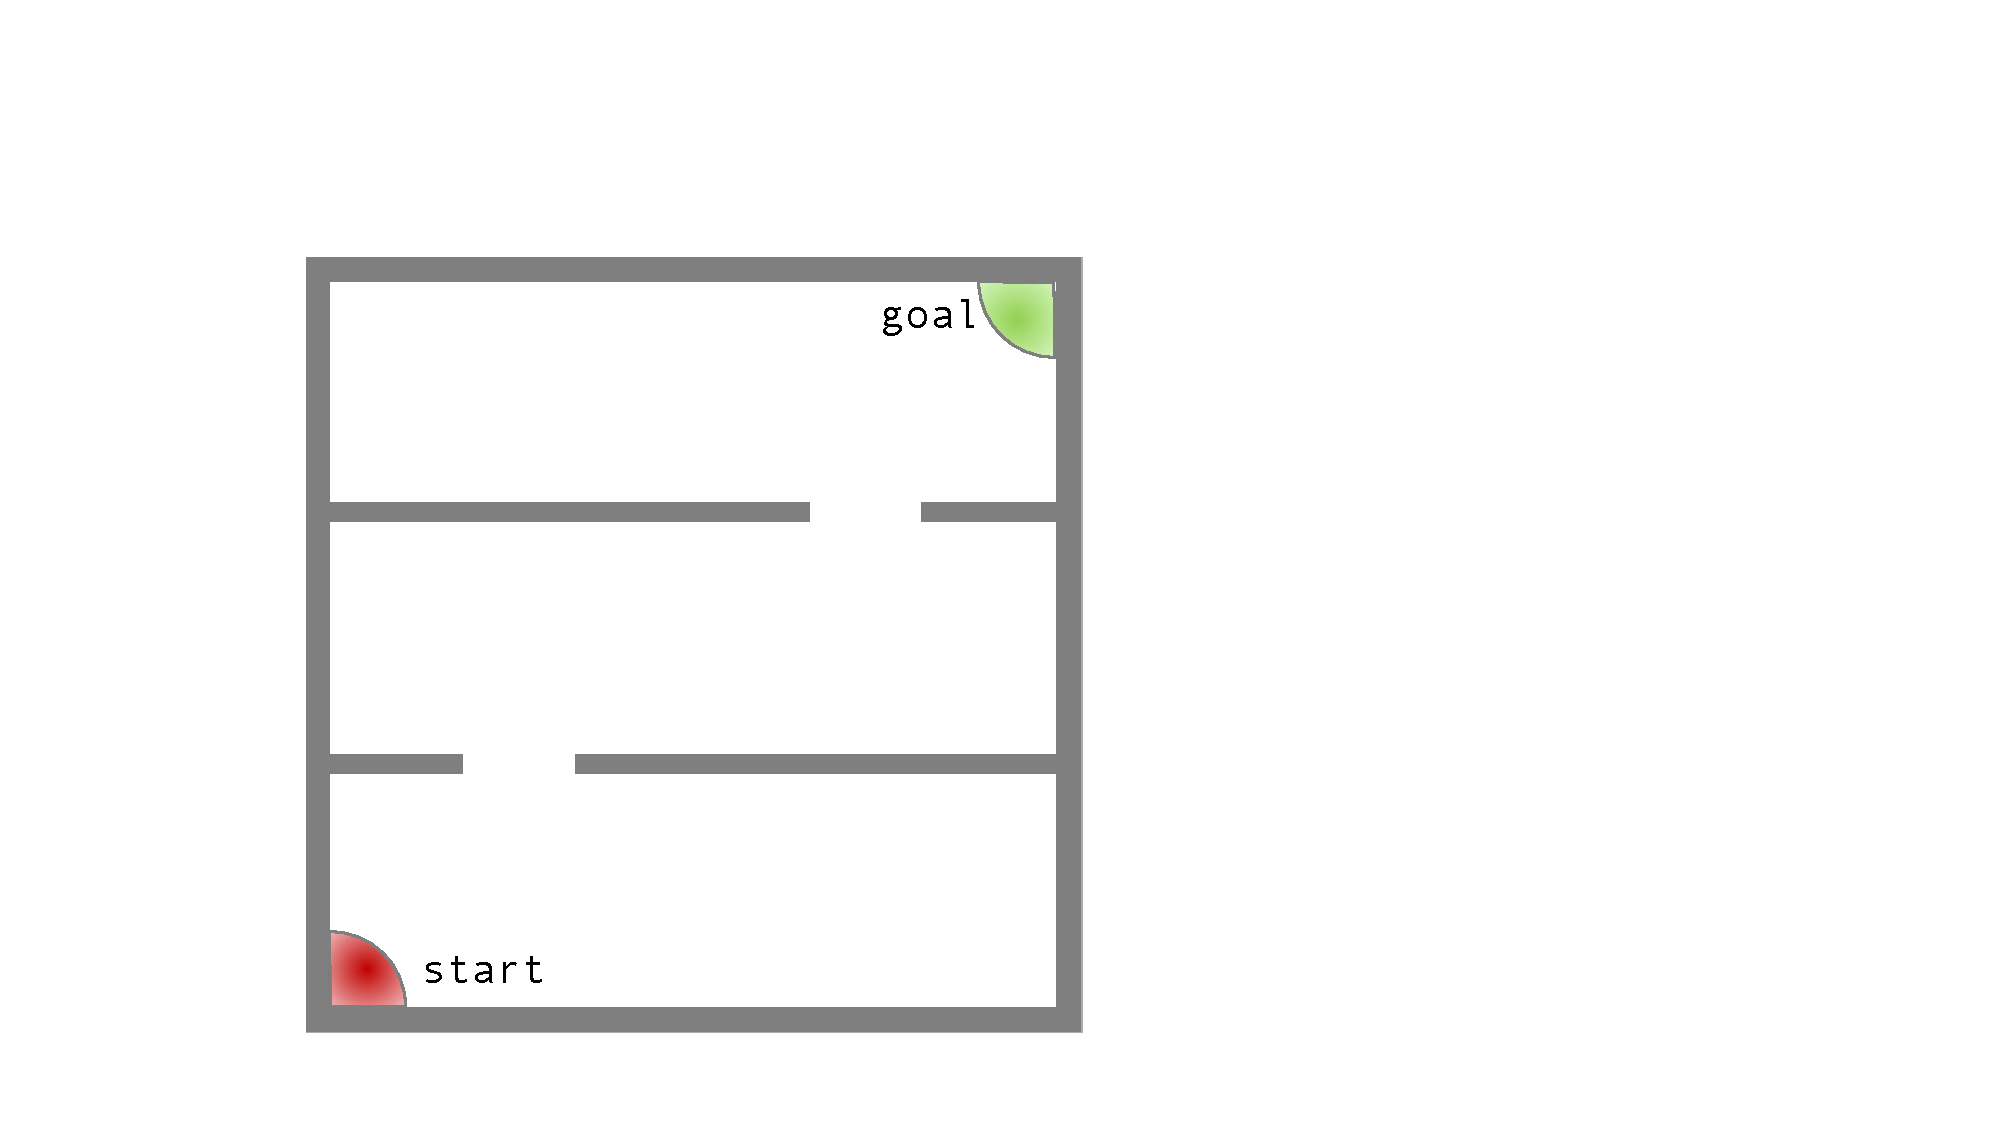
\includegraphics[trim=0.0cm 0.2cm 0.0cm 0.2cm,clip=true,height=2.6cm, width=2.0cm]{images/rooms2.pdf}
    \caption{}
  \end{subfigure}
  \begin{subfigure}[b]{0.27\textwidth}
    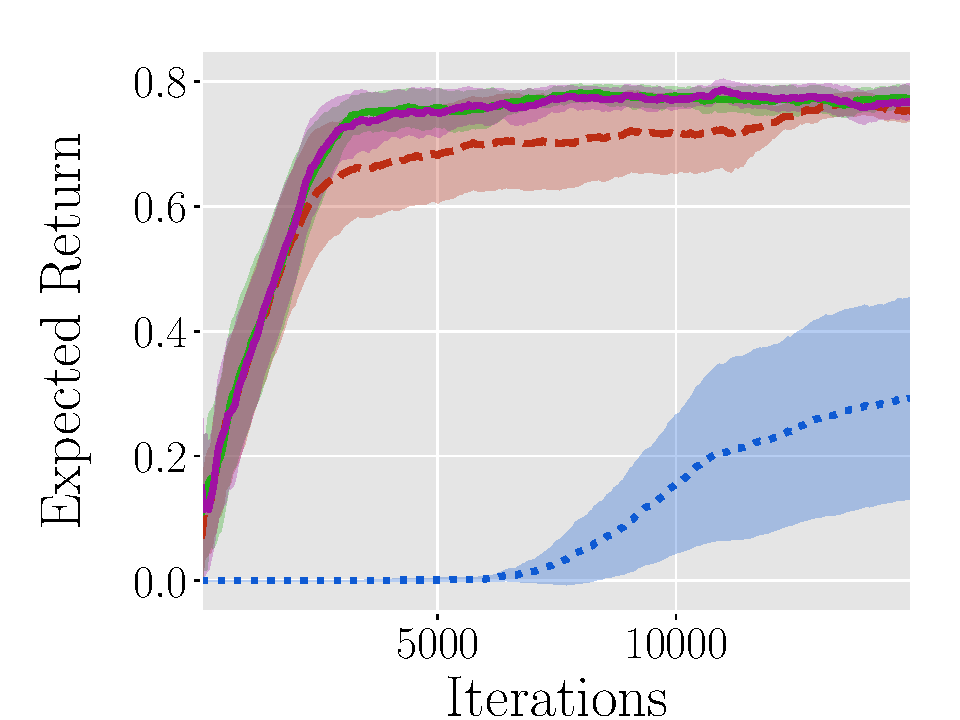
\includegraphics[trim=0.5cm 0cm 1.8cm 1.3cm,clip=true,height=2.9cm]{images/three-room/lrev.pdf}
    \caption{}
  \end{subfigure}
    \begin{subfigure}[b]{0.27\textwidth}
    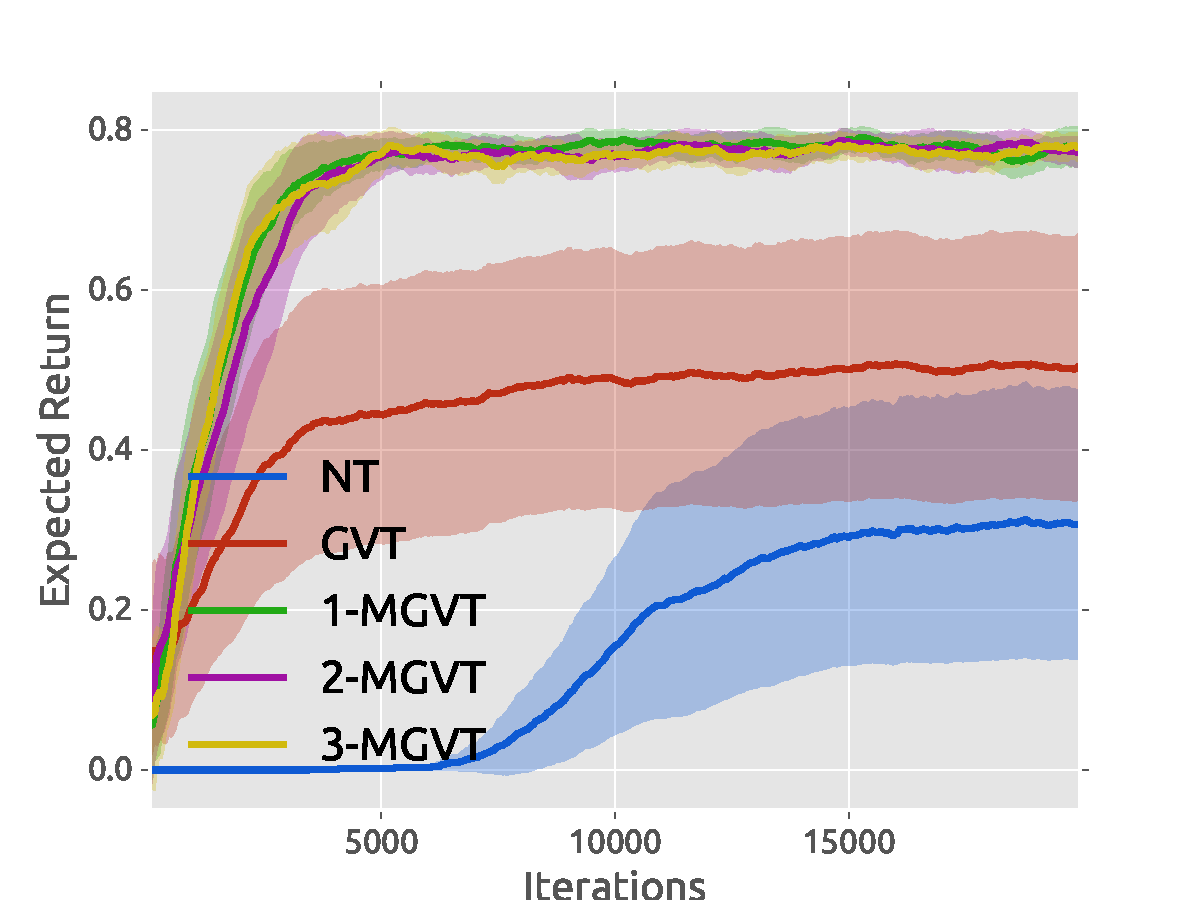
\includegraphics[trim=0.5cm 0cm 1.6cm 1.3cm,clip=true,height=2.9cm]{images/three-room-gen/lrev.pdf}
    \caption{}
  \end{subfigure}
    \begin{subfigure}[b]{0.27\textwidth}
    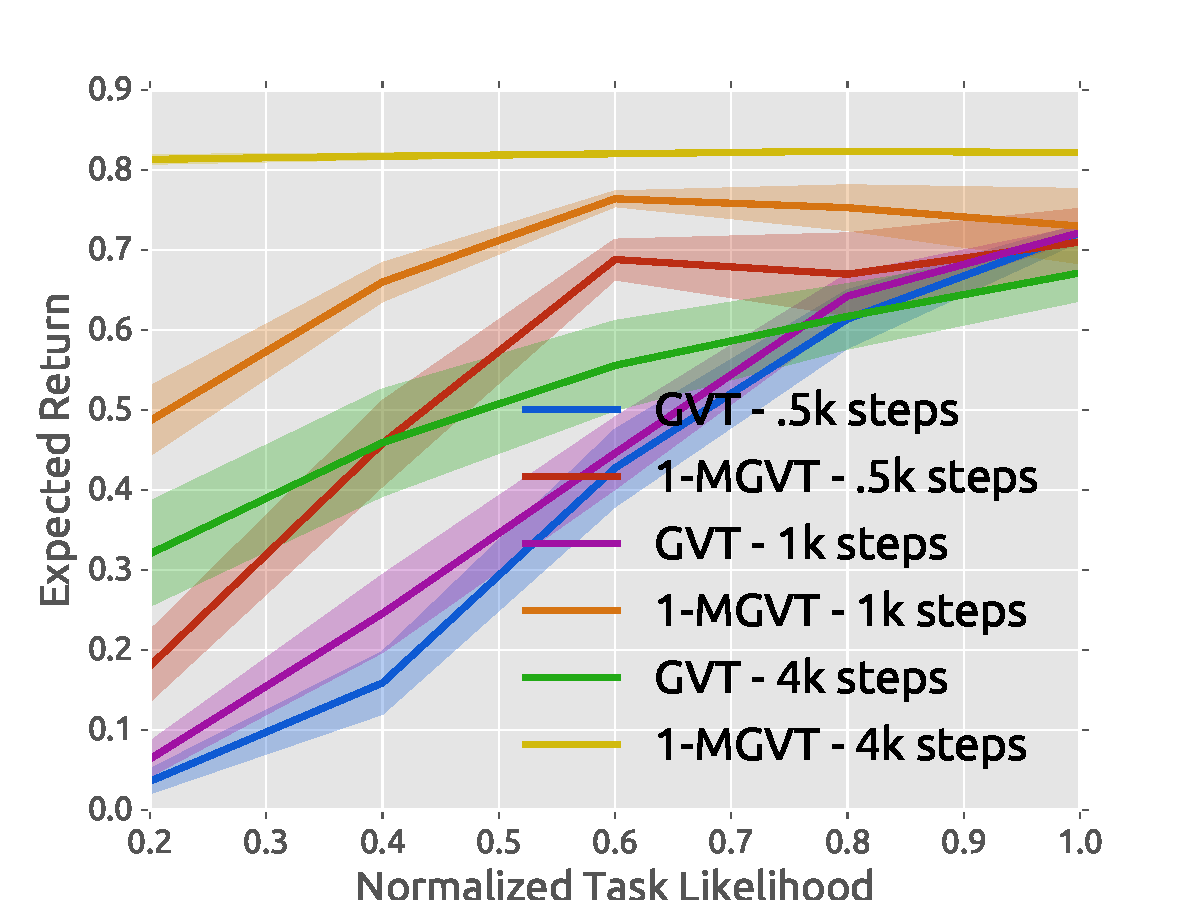
\includegraphics[trim=0.5cm 0cm 1.6cm 1.3cm,clip=true,height=2.9cm]{images/likelihood/lrew.pdf}
    \caption{}
  \end{subfigure}
  \caption{(a) the rooms environment, (b) transfer from $10$ source tasks with both doors moving, (c) transfer from $10$ source tasks with only one door moving, and (d) transfer performance as a function of how likely the target task is according to the prior.}
  \label{fig:dipfdbsgraphplots}
\end{figure*}

In order to prove that our guesses are correct, we generate a set of $50$ source tasks for the three-room environment of Fig. \ref{} by sampling both door positions uniformly, and solve all of them by directly minimizing the TD error as presented in Sec. \ref{sec:td}. In order to make sure that their solutions are accurate enough, we allow sampling the initial state uniformly in the environment and run until convergence. Then, we use our algorithms to transfer from $10$ source tasks sampled from the previously generated set. The average return over the last $50$ learning episodes as a function of the number of iterations is shown in Fig. \ref{}. Each curve is the result of $20$ independent runs, each resampling the target and source tasks. $95\%$ confidence intervals are shown. Further details on the parameters adopted in this experiment are given in App. \ref{}. As expected, the no-transfer (NT) algorithm fails at learning the task in so few iterations due to the limited exploration provided by an $\epsilon$-greedy policy. On the other hand, all our algorithms achieve a significant speed-up and are able to converge to the optimal performance in few iterations, with GVT being slightly slower. Interestingly, we notice that there is no advantage in adopting more than $1$ component for the posterior in MGVT. This is intuitive since, when the algorithm quickly figures out which task is being solved, it will move all components in the same direction.

To better understand the differences between GVT and MGVT, we now consider transferring from a slightly different distribution than the one from which target tasks are drawn. We generate again $50$ source tasks but this time with the bottom door fixed in the center and the other one moving. Then, we repeat the previous experiment, allowing both doors to move when sampling target tasks. The results are shown in Fig. \ref{}. Interestingly, MGVT seems almost unaffected by this change, proving that is has sufficient representation power to generalize to slightly different task distributions. The same does not hold for GVT, which now is not able to solve many of the sampled target tasks,thus the very high variance. This proves again that assuming Gaussian distributions can pose severe limitations in our transfer settings.

Finally, we analyze the transfer performance as a function of how likely the target task is according to the prior. We consider a two-room version of the environment of Fig. \ref{}. Differently from before, we generate tasks by sampling the door position from a Gaussian with mean $5$, and standard deviation $1.8$, so that tasks where the door is near the sides are very unlikely. Fig. \ref{} shows the performance reached by GVT and MGVT with $1$ component at fixed iterations as a function of how likely the target task is according to such distribution. As expected GVT achieves poor performance on very unlikely tasks, even after many iterations. In fact, estimating a single Gaussian distribution definitely entails some information loss, especially about the unlikely tasks. On the other hand, MGVT keeps such information and, consequently, performs much better. Perhaps not surprisingly, MGVT reaches the optimal performance in $4k$ iterations no matter what task is being solved.

\subsection{Classic Control} \label{sec:cc}

To evaluate the performance of our transfer algorithms in more common benchmarks, we chose to use the well-known classic control environments: Cartpole and Mountain Car as defined in \citep{sutton1998reinforcement}. In the case of Cartpole we generated $20$ source tasks by uniformly sampling the cart mass, the pole mass and length. Instead, for Mountain Car, we generated the $20$ sources by uniformly sampling the base speed of the car. We kept a discount factor of $\gamma=0.99$ for both environments. Moreover, to train the source tasks we chose to use a Multilayer Perceptron (MLP) as approximator. We trained all source tasks until convergence and to transfer, in both settings, we used GVT and 1-MGVT choosing randomly $10$ of the trained sources. Analogously to Sec. \ref{sec:gw}, in Fig. \ref{} and \ref{} we show the expected return---as the average of the last $50$ episodes of lerning---of transfer for $20$ independent runs randomizing the sources and target tasks. In Fig. \ref{}, that corresponds to Cartpole, it is easily noticeable a near-optimal jump-start, in both GVT and 1-MGVT, that during the following iterations converges to the optimal performance. Furthermore, transfer in Mountain Car as shown in Fig. \ref{}, a more complicated task than Cartpole, causes GVT to struggle to solve the target task but 1-MGVT reaches convergence, within the same number of iterations, to the optimal performances.

\subsection{Maze Navigation} \label{sec:mn}

\begin{figure*}[t]
  \begin{subfigure}[b]{0.15\textwidth}
    
\includegraphics[trim=0.0cm 0.0cm 0.0cm 0.0cm,clip=true,height=2.6cm, width=2.0cm]{images/maze/maze6.png}
    \caption{}
  \end{subfigure}
  \begin{subfigure}[b]{0.27\textwidth}
    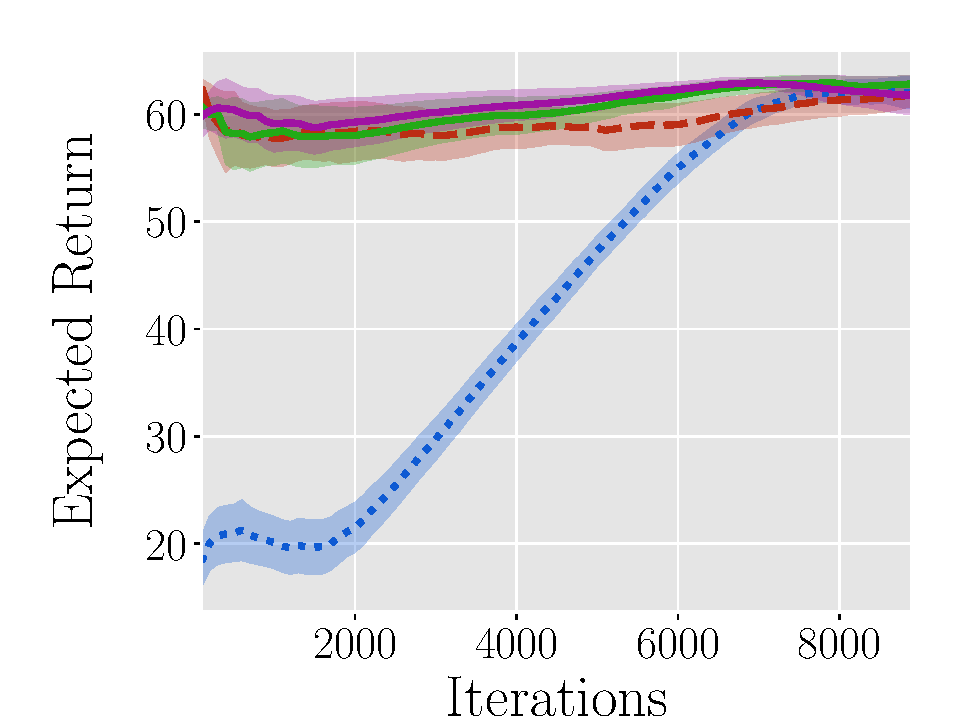
\includegraphics[trim=0.5cm 0cm 1.8cm 1.3cm,clip=true,height=2.9cm]{images/cartpole/lrev.pdf}
    \caption{}
  \end{subfigure}
    \begin{subfigure}[b]{0.27\textwidth}
    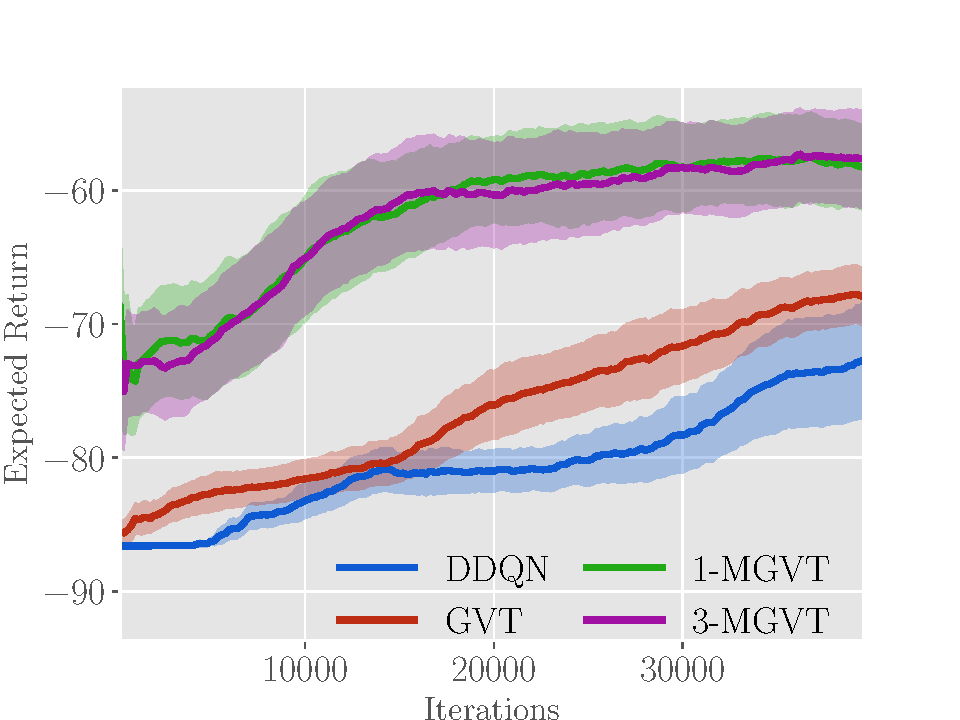
\includegraphics[trim=0.5cm 0cm 1.6cm 1.3cm,clip=true,height=2.9cm]{images/mountaincar/lrev.pdf}
    \caption{}
  \end{subfigure}
    \begin{subfigure}[b]{0.27\textwidth}
    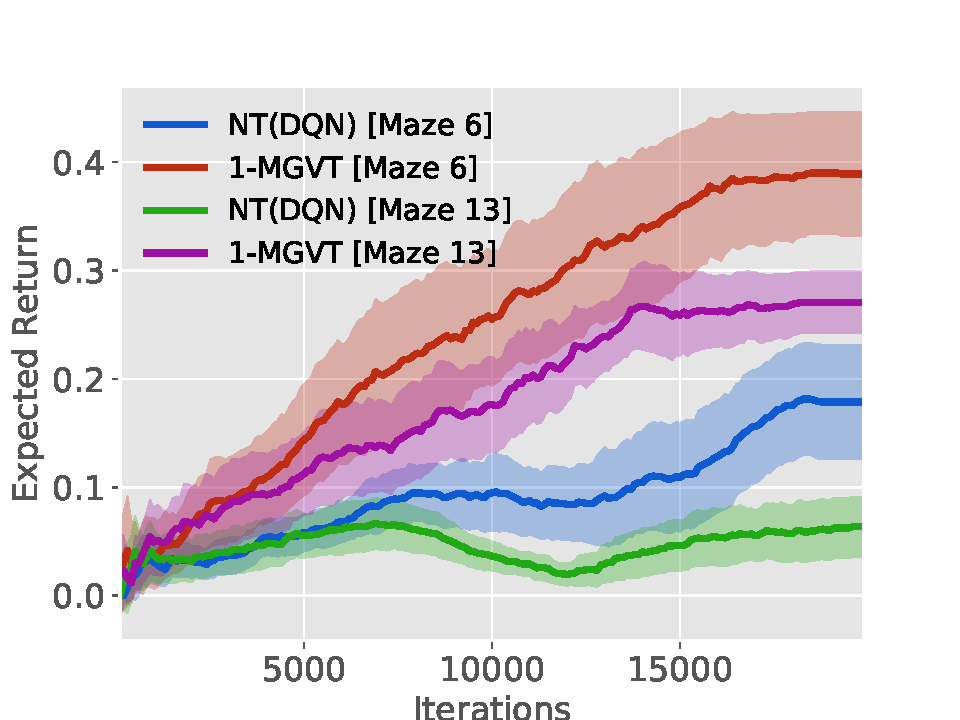
\includegraphics[trim=0.5cm 0cm 1.6cm 1.3cm,clip=true,height=2.9cm]{images/maze/lrev.pdf}
    \caption{}
  \end{subfigure}
  \caption{(a) Sample Maze (Maze 6), (b) transfer from $10$ sources in Cartpole, (c) transfer from $10$ source tasks in Mountain Car, and (d) transfer from $10$ sources in Mazes 6 and 13---see App. \ref{}.}
  \label{fig:ccmazeplots}
\end{figure*}

For this setting we propose a maze environment, such as those in Fig. \ref{}, for a robotic agent to navigate. We created a set of 20 mazes---see App \ref{}---of size $10\times10$ with continuous space within which we ensured four groups: each group with the goal position in one of the corners of the maze. In order to simulate a robotic agent, we set an action space that allows to control the linear and angular motion by a fixed distance of $0.5$ (\emph{move forward}) and a fixed angle of $\pm 22.5º$ (\emph{rotate counter- and clockwise}). Moreover, we enhanced the state space to include, in addition to the absolute position and orientation, a set of distance measurements to the nearest obstacles from the agent's perspective with maximum range of $2$ and a field of vision of $9$ equally-spaced directions in $[-90,90º]$ relative to its orientation. In this way, we provide the agent with information that a robot would normally collect from LIDARs, sonars and other sensors alike. Finally, in the same field of perception, we provide a boolean vector indicating whether the goal is within the range of observation. Regarding rewards, the agent gets 1 whenever it enters the goal area and 0 in any other situation and the MDP has a discount factor of $\gamma = 0.99$.

The main motivation for this set-up is that a robot is able to exploit locally-sensed information in addition to its estimation of the actual position---as opposed to the Rooms problem presented above---and it is such information that the robotic agent could learn to use and, also, exploit in different maze configurations leveraging its previous experience. Moreover, simple variations in the maze structure could, potentially, produce big differences in the value function with respect to the ones seen in previous tasks which makes the setting suitable to assess how robust our algorithm is to negative transfer.

The mazes were solved using Deep Q Networks (DQN) [] \todo{cite DQN?} with an MLP with hidden layers $32\times32$ and, in order to perform the knowledge transfer, the target maze would be excluded from the source tasks given to the algorithm. Finally, the 1-MGVT algorithm was used to solve the target tasks---Mazes 6 and 13. As before, $20$ independent runs with randomized sources to transfer are averaged and shown in Fig. \ref{}, in this case $5$ source tasks were used for each trial. While these mazes pose a challenge for our algorithm, we can see that 1-MGVT is capable to still capture useful information from the sources and adapt to the target mazes which is demonstrated by the increased slope in the learning curve. \todo{actually, decide how to improve these results}

\section{Related Works}

Our approach is mostly related to \cite{lazaric2010bayesian}. Although we both assume the tasks to share similarities in their value functions, \cite{lazaric2010bayesian} consider only linear approximators and adopt a hierarchical Bayesian model of the corresponding weights' distribution, which is assumed Gaussian. On the other hand, our variational approximation allows for more general distribution families and can be combined with non-linear approximators. Furthermore, \cite{lazaric2010bayesian} propose a Dirichlet process model for the case where weights cluster into different classes, which relates to our mixture formulation and proves again the importance of capturing more complicated task distributions. In \cite{wilson2007multi}, the authors propose a hierarchical Bayesian model for the distribution over tasks. Differently from our approach and \cite{lazaric2010bayesian}, they consider a distribution over transition probabilities and rewards, rather than value functions. In the same spirit of our method, they consider a Thompson sampling-based procedure which, at each iteration, samples a new task from the posterior and solves it. However, \cite{wilson2007multi} consider only finite MDPs, which poses a severe limitation on the algorithm's applicability. On the contrary, our approach can handle high-dimensional tasks. In \cite{doshi2016hidden}, the authors consider a family of tasks whose dynamics are governed by some hidden parameters and use Gaussian processes (GPs) to model such dynamics across tasks. Recently, \cite{killian2017robust} extended this approach by replacing GPs with Bayesian neural networks, so as to obtain a more scalable approach.\todo{More comments about HiP-MDPs? Should we discuss more related works?}

In the RL community, our approach is related to value function randomization\cite{osband2014generalization}, which extends the well-known LSTD \cite{boyan1999least} by adopting Bayesian linear regression to model the uncertainty over the predicted value function weights, and use that to perform a form of Thompson sampling. Such approach was recently extended by \cite{azizzadenesheli2018efficient}, where the approximator is replaced by a Bayesian neural network, leading to an algorithm capable of solving much more complicated problems. Both these algorithms rely on the Gaussian assumption and, since they work in plain RL settings, have no informative prior available. On the other hand, our variational approximation allows more complex distributions (e.g., mixtures) to be adopted, while knowledge from the source tasks allows us to learn very informative priors.

\section{Conclusion}

{\small 
\bibliography{biblio.bib}
\bibliographystyle{plain}
}

\newpage
\appendix

\section{Proofs}

\thmm*
\begin{proof}
We begin by noticing that:
\begin{align*}
\norm{Q^*-\wt{Q}}_{\nu,p}^p =\ & \norm{TQ^* - \wt{T}\wt{Q}}_{\nu,p}^p \\ =\ &
\norm{TQ^* - \wt{T}Q^* + \wt{T}Q^* - \wt{T}\wt{Q}}_{\nu,p}^p \\ \leq\ &
\norm{TQ^* - \wt{T}Q^*}_{\nu,p}^p + \norm{\wt{T}Q^* - \wt{T}\wt{Q}}_{\nu,p}^p \\ \leq\ &
\norm{TQ^* - \wt{T}Q^*}_{\nu,p}^p + \gamma\norm{Q^* - \wt{Q}}_{\nu,p}^p
\end{align*}
where the first inequality follows from Minkowsky's inequality and the second one from the contraction property of the mellow Bellman operator. This implies that:
\begin{align} \label{eq:mm1}
\norm{Q^*-\wt{Q}}_{\nu,p}^p \leq \frac{1}{1-\gamma}\norm{TQ^* - \wt{T}Q^*}_{\nu,p}^p
\end{align}
Let us bound the norm on the right-hand side separately. In order to do that, we will bound the function $\abs{TQ^*(s,a) - \wt{T}Q^*(s,a)}$ point-wisely for any state $s,a$. By applying the definition of the optimal and mellow Bellman operators, we obtain:
\begin{align} \label{eq:mm5}
\abs{TQ^*(s,a) - \wt{T}Q^*(s,a)} =\ & \abs{R(s,a) + \gamma\mathbb{E}\left[\max_{a'}Q^*(s',a')\right] - R(s,a) - \gamma\mathbb{E}\left[\mm_{a'}Q^*(s',a')\right]}\notag \\ =\ & \gamma\abs{\mathbb{E}\left[\max_{a'}Q^*(s',a')\right] - \mathbb{E}\left[\mm_{a'}Q^*(s',a')\right]}\notag \\ \leq\ & \gamma\mathbb{E}\left[\abs{\max_{a'}Q^*(s',a') - \mm_{a'}Q^*(s',a')}\right]
\end{align}
Thus, bounding this quantity reduces to bounding $\abs{\max_{a}Q^*(s,a) - \mm_{a}Q^*(s,a)}$ point-wisely for any $s$. Recall that applying the mellow-max is equivalent to computing an expectation under a Boltzmann distribution with inverse temperature $\beta_{\kappa}$ induced by $\kappa$ \cite{}\todo{Cite MM}. Thus, we can write:
\begin{align} \label{eq:mm2}
\abs{\max_a Q^*(s,a) - \mm_a Q^*(s,a)} =\ & \abs{\sum_a \pi^*(a|s)Q^*(s,a) - \sum_a \pi_{\beta_{\kappa}}(a|s)Q^*(s,a)}\notag\\ =\ & \abs{\sum_a Q^*(s,a) \left( \pi^*(a|s) - \pi_{\beta_{\kappa}}(a|s)  \right)}\notag\\ \leq\ & \sum_a \abs{Q^*(s,a)} \abs{\pi^*(a|s) - \pi_{\beta_{\kappa}}(a|s)}\notag\\ \leq\ & \frac{R_{max}}{1-\gamma}\sum_a\abs{\pi^*(a|s) - \pi_{\beta_{\kappa}}(a|s)}
\end{align}
where $\pi^*$ is the optimal (deterministic) policy w.r.t. $Q^*$ and $\pi_{\beta_{\kappa}}$ is the Boltzmann distribution induced by $Q^*$ with inverse temperature $\beta_{\kappa}$:
\begin{align*}
\pi_{\beta}(a|s) = \frac{e^{\beta_{\kappa} Q^*(s,a)}}{\sum_{a'}e^{\beta_{\kappa} Q^*(s,a')}}
\end{align*}
Denote by $a_1(s)$ the optimal action for state $s$ under $Q^*$. We can then write:
\begin{align} \label{eq:mm3}
\sum_a\abs{\pi^*(a|s) - \pi_{\beta_{\kappa}}(a|s)} =\ & \abs{\pi^*(a_1(s)|s) - \pi_{\beta_{\kappa}}(a_1(s)|s)} + \sum_{a \neq a_1(s)}\abs{\pi^*(a|s) - \pi_{\beta_{\kappa}}(a|s)}\notag\\ =\ & \abs{1 - \pi_{\beta_{\kappa}}(a_1(s)|s)} + \sum_{a \neq a_1(s)}\abs{\pi_{\beta_{\kappa}}(a|s)}\notag\\ =\ & 2\abs{1 - \pi_{\beta_{\kappa}}(a_1(s)|s)}
\end{align}
Finally, let us bound this last term:
\begin{align} \label{eq:mm4}
\abs{1 - \pi_{\beta_{\kappa}}(a_1(s)|s)} =\ & \abs{1 - \frac{e^{\beta_{\kappa} Q^*(s,a_1(s))}}{\sum_{a'}e^{\beta_{\kappa} Q^*(s,a')}}}\notag\\ =\ & \abs{1 - \frac{e^{\beta_{\kappa} \left( Q^*(s,a_1(s)) - Q^*(s,a_2(s)) \right)}}{\sum_{a'}e^{\beta_{\kappa} \left( Q^*(s,a') - Q^*(s,a_2(s))\right)}}}\notag\\ =\ & \abs{1 - \frac{e^{\beta_{\kappa} g(s)}}{\sum_{a'}e^{\beta_{\kappa} \left( Q^*(s,a') - Q^*(s,a_2(s))\right)}}}\notag\\ =\ & \abs{1 - \frac{e^{\beta_{\kappa} g(s)}}{e^{\beta_{\kappa} g(s)} + \sum_{a' \neq a_1(s)}e^{\beta_{\kappa} \left( Q^*(s,a') - Q^*(s,a_2(s))\right)}}}\notag\\ \leq & \abs{1 - \frac{e^{\beta_{\kappa} g(s)}}{e^{\beta_{\kappa} g(s)} + \abs{\mathcal{A}}}}\notag\\ = & \abs{\frac{1}{1 + \frac{1}{\abs{\mathcal{A}}}e^{\beta_{\kappa} g(s)}}}
\end{align}
Combining Eq. \eqref{eq:mm2}, \eqref{eq:mm3}, and \eqref{eq:mm4}, we obtain:
\begin{align*}
\abs{\max_a Q(s,a) - \mm_a Q(s,a)} \leq\ \frac{2 R_{max}}{1-\gamma}\abs{\frac{1}{1 + \frac{1}{\abs{\mathcal{A}}}e^{\beta_{\kappa} g(s)}}}
\end{align*}
Finally, using Eq. \eqref{eq:mm5} we get:
\begin{align*}
\abs{TQ^*(s,a) - \wt{T}Q^*(s,a)} \leq \frac{2\gamma R_{max}}{1-\gamma}\abs{\frac{1}{1 + \frac{1}{\abs{\mathcal{A}}}e^{\beta_{\kappa} g(s)}}}
\end{align*}
Taking the norm and plugging this into Eq. \eqref{eq:mm1} concludes the proof.
\end{proof}

\begin{lemma}
Let $p$ and $\nu$ denote probability measures over $Q$-functions and state-action pairs, respectively. Assume $Q^*$ is the unique fixed-point of the optimal Bellman operator $T$. Then, for any $\delta > 0$, with probability at least $1 - \delta$ over the choice of a $Q$-function $Q$, the following holds:
\begin{equation}
\norm{Q - Q^*}_{\nu}^2 \leq \frac{\mathbb{E}_p\left[ \norm{B(Q)}_{\nu}^2 \right]}{(1-\gamma)\delta}
\end{equation}
\end{lemma}
\begin{proof}
First notice that:
\begin{align*}
\norm{Q - Q^*} =\ & \norm{Q + TQ - TQ - TQ^*}\\ \leq\ & \norm{Q - TQ} + \norm{TQ - TQ^*}\\ \leq\ & \norm{Q - TQ} + \gamma\norm{Q - Q^*}\\ =\ & \norm{B(Q)} + \gamma\norm{Q - Q^*}
\end{align*}
which implies that:
\begin{align*}
\norm{Q - Q^*} \leq\ \frac{1}{1-\gamma}\norm{B(Q)}
\end{align*}
Then we can write:
\begin{align*}
P\left( \norm{Q - Q^*} > \epsilon \right) \leq P\left(\norm{B(Q)} > \epsilon (1-\gamma)\right) \leq \frac{\mathbb{E}_p\left[ \norm{B(Q)}_{\nu}^2 \right]}{(1-\gamma)\epsilon}
\end{align*}
Settings the right-hand side equal to $\delta$ and solving for $\epsilon$ concludes the proof.
\end{proof}

\begin{corollary}\label{cor:diff-q}
Let $p$ and $\nu$ denote probability measures over $Q$-functions and state-action pairs, respectively. Assume $\wt{Q}$ is the unique fixed-point of the mellow Bellman operator $\wt{T}$. Then, for any $\delta > 0$, with probability at least $1 - \delta$ over the choice of a $Q$-function $Q$, the following holds:
\begin{equation}
\norm{Q - \wt{Q}}_{\nu}^2 \leq \frac{\mathbb{E}_p\left[ \norm{\wt{B}(Q)}_{\nu}^2 \right]}{(1-\gamma)\delta}
\end{equation}
\end{corollary}

\begin{lemma}\label{lemma:l2}
Assume $Q$-functions belong to a parametric space of functions bounded by $\frac{R_{max}}{1-\gamma}$. Let $p$ and $q$ be arbitrary distributions over the parameter space $\mathcal{W}$, and $\nu$ be a probability measure over $\mathcal{S}\times\mathcal{A}$. Consider a dataset $D$ of $N$ samples and define $v(\bm{w}) \triangleq \mathbb{E}_{\nu}\left[Var_{\mathcal{P}}\left[b(\bm{w})\right]\right]$. Then, for any $\delta > 0$, with probability at least $1-\delta$, the following two inequalities hold simultaneously:
\begin{equation}\label{eq:lemma2-1}
\mathbb{E}_q\left[ \norm{B(\bm{w})}_{\nu}^2 \right ] \leq \mathbb{E}_q\left[ \norm{B(\bm{w})}_D^2 \right] - \mathbb{E}_q\left[ v(\bm{w}) \right] + \frac{\lambda}{N} KL(q||p) + 4\frac{R_{max}^2}{(1-\gamma)^2}\sqrt{\frac{\log\frac{2}{\delta}}{2N}}
\end{equation}
\begin{equation}\label{eq:lemma2-2}
\mathbb{E}_q\left[ \norm{B(\bm{w})}_D^2 \right] \leq \mathbb{E}_q\left[ \norm{B(\bm{w})}_{\nu}^2 \right ] + \mathbb{E}_q\left[ v(\bm{w}) \right] + \frac{\lambda}{N} KL(q||p) + 4\frac{R_{max}^2}{(1-\gamma)^2}\sqrt{\frac{\log\frac{2}{\delta}}{2N}}
\end{equation}
\end{lemma}
\begin{proof}
From Hoeffding's inequality we have:
\begin{align*}
P\left( \abs{\mathbb{E}_{\nu,\mathcal{P}}\left[\norm{B(\bm{w})}_D^2\right] - \norm{B(\bm{w})}_D^2} > \epsilon \right) \leq 2exp\left( -\frac{2N\epsilon^2}{\left(2\frac{R_{max}}{1-\gamma}\right)^4} \right)
\end{align*}
which implies that, for any $\delta>0$, with probability at least $1-\delta$:
\begin{align*}
\abs{\mathbb{E}_{\nu,\mathcal{P}}\left[\norm{B(\bm{w})}_D^2\right] - \norm{B(\bm{w})}_D^2} \leq 4\frac{R_{max}^2}{(1-\gamma)^2}\sqrt{\frac{\log\frac{2}{\delta}}{2N}}
\end{align*}
Under independence assumptions, the expected TD error can be re-written as:
\begin{align*}
\mathbb{E}_{\nu,\mathcal{P}}\left[\norm{B(\bm{w})}_D^2\right] =\ & \mathbb{E}_{\nu,\mathcal{P}}\left[\frac{1}{N}\sum_{i=1}^N (r_i + \gamma \mm_{a'} Q_{\bm{w}}(s_i',a') - Q_{\bm{w}}(s_i,a_i))^2\right]\\ =\ & \mathbb{E}_{\nu,\mathcal{P}}\left[(R(s,a) + \gamma \mm_{a'} Q_{\bm{w}}(s',a') - Q_{\bm{w}}(s,a))^2\right]\\ =\ & \mathbb{E}_{\nu}\left[\mathbb{E}_{\mathcal{P}}\left[b(\bm{w})^2\right]\right]\\ =\ & \mathbb{E}_{\nu}\left[Var_{\mathcal{P}}\left[b(\bm{w})\right] + \mathbb{E}_{\mathcal{P}}\left[b(\bm{w})\right]^2\right]\\ =\ & v(\bm{w}) + \norm{B(\bm{w})}_{\nu}^2
\end{align*}
where $v(\bm{w}) \triangleq \mathbb{E}_{\nu}\left[Var_{\mathcal{P}}\left[b(\bm{w})\right]\right]$. Thus:
\begin{align}\label{eq:hoeff}
\abs{\norm{B(\bm{w})}_{\nu}^2 + v(\bm{w}) - \norm{B(\bm{w})}_D^2} \leq 4\frac{R_{max}^2}{(1-\gamma)^2}\sqrt{\frac{\log\frac{2}{\delta}}{2N}}
\end{align}
From the change of measure inequality \cite{}\todo{Find a reference for this}, we have that, for any measurable function $f(\bm{w})$ and any two probability measures $p$ and $q$:
\begin{align*}
\log\mathbb{E}_p\left[e^{f(\bm{w})}\right] \geq \mathbb{E}_q\left[ f(\bm{w}) \right] - KL(q||p)
\end{align*}
Thus, multiplying both sides of \eqref{eq:hoeff} by $\lambda^{-1}N$ and applying the change of measure inequality with $f(\bm{w}) = \lambda^{-1}N\abs{\norm{B(\bm{w})}_{\nu}^2 + v(\bm{w}) - \norm{B(\bm{w})}_D^2}$, we obtain:
\begin{align*}
\mathbb{E}_q\left[ f(\bm{w}) \right] - KL(q||p) \leq \log\mathbb{E}_p\left[e^{f(\bm{w})}\right] \leq 4\frac{R_{max}^2 \lambda^{-1}N}{(1-\gamma)^2}\sqrt{\frac{\log\frac{2}{\delta}}{2N}}
\end{align*}
where the second inequality holds since the right-hand side of \eqref{eq:hoeff} does not depend on $\bm{w}$. Finally, we can explicitly write:
\begin{align*}
\mathbb{E}_q\left[ \abs{\norm{B(\bm{w})}_{\nu}^2 + v(\bm{w}) - \norm{B(\bm{w})}_D^2} \right] \leq \frac{\lambda}{N} KL(q||p) + 4\frac{R_{max}^2}{(1-\gamma)^2}\sqrt{\frac{\log\frac{2}{\delta}}{2N}}
\end{align*}
from which the lemma follows straightforwardly.
\end{proof}

\begin{lemma}\label{lemma:general-bound}
Let $p$ be a prior distribution over the parameter space $\mathcal{W}$, and $\nu$ be a probability measure over $\mathcal{S}\times\mathcal{A}$. Assume $\wh{\xi}$ is the minimizer of $ELBO(\xi) = \mathbb{E}_{q_{\xi}}\left[ \norm{B(\bm{w})}_D^2 \right] + \frac{\lambda}{N} KL({q_{\xi}}||p)$ for a dataset $D$ of $N$ samples. Define $v(\bm{w}) \triangleq \mathbb{E}_{\nu}\left[Var_{\mathcal{P}}\left[b(\bm{w})\right]\right]$. Then, for any $\delta > 0$, with probability at least $1-\delta$:
\begin{align*}
\mathbb{E}_{q_{\wh{\xi}}}\left[ \norm{B(\bm{w})}_{\nu}^2 \right ] \leq \inf_{\xi \in \Xi}\left\{ \mathbb{E}_{q_{\xi}}\left[ \norm{B(\bm{w})}_{\nu}^2 \right ] + \mathbb{E}_{q_{\xi}}\left[ v(\bm{w}) \right] + 2\frac{\lambda}{N} KL({q_{\xi}}||p) \right\} + 2\frac{R_{max}^2}{(1-\gamma)^2}\sqrt{\frac{\log\frac{2}{\delta}}{N}}
\end{align*}
\end{lemma}
\begin{proof}
Let us use Lemma \ref{lemma:l2} for the specific choice $q=q_{\wh{\xi}}$. From Eq. \eqref{eq:lemma2-1}, we have:
\begin{align*}
\mathbb{E}_{q_{\wh{\xi}}}\left[ \norm{B(\bm{w})}_{\nu}^2 \right ] \leq\ & \mathbb{E}_{q_{\wh{\xi}}}\left[ \norm{B(\bm{w})}_D^2 \right] - \mathbb{E}_{q_{\wh{\xi}}}\left[ v(\bm{w}) \right] + \frac{\lambda}{N} KL({q_{\wh{\xi}}}||p) + 4\frac{R_{max}^2}{(1-\gamma)^2}\sqrt{\frac{\log\frac{2}{\delta}}{2N}}\\ \leq\ & \mathbb{E}_{q_{\wh{\xi}}}\left[ \norm{B(\bm{w})}_D^2 \right] + \frac{\lambda}{N} KL({q_{\wh{\xi}}}||p) + 4\frac{R_{max}^2}{(1-\gamma)^2}\sqrt{\frac{\log\frac{2}{\delta}}{2N}}\\ =\ & \inf_{\xi \in \Xi}\left\{ \mathbb{E}_{q_{\xi}}\left[ \norm{B(\bm{w})}_D^2 \right] + \frac{\lambda}{N} KL({q_{\xi}}||p) \right\} + 4\frac{R_{max}^2}{(1-\gamma)^2}\sqrt{\frac{\log\frac{2}{\delta}}{2N}}
\end{align*}
where the second inequality holds since $v(\bm{w}) > 0$, while the equality holds from the definition of $\wh{\xi}$. We can now use Eq. \eqref{eq:lemma2-2} to bound $\mathbb{E}_{q_{\xi}}\left[ \norm{B(\bm{w})}_D^2 \right]$, thus obtaining:
\begin{align*}
\mathbb{E}_{q_{\wh{\xi}}}\left[ \norm{B(\bm{w})}_{\nu}^2 \right ] \leq \inf_{\xi \in \Xi}\left\{ \mathbb{E}_{q_{\xi}}\left[ \norm{B(\bm{w})}_{\nu}^2 \right ] + \mathbb{E}_{q_{\xi}}\left[ v(\bm{w}) \right] + 2\frac{\lambda}{N} KL({q_{\xi}}||p) \right\} + 2\frac{R_{max}^2}{(1-\gamma)^2}\sqrt{\frac{\log\frac{2}{\delta}}{N}}
\end{align*}
This concludes the proof.
\end{proof}

\begin{theorem}\label{th:main-gaussian}
Fix a target task $\tau$ a let $\wt{Q}$ be the fixed-point of the corresponding mellow Bellman operator. Assume linearly parameterized value functions $Q_{\bm{w}}(s,a)=\bm{w}^T\bm{\phi}(s,a)$ with bounded weights $\bm{w}\leq w_{max}$ and uniformly bounded features $\bm{\phi}(s,a)\leq \phi_{\max}$. Consider the Gaussian version of Alg. \ref{alg:transfer} with prior $p(\bm{w}) =\mathcal{N}(\bm{\mu}_p,\bm{\Sigma}_p)$ and denote by $(\wh{\bm{\mu}},\wh{\bm{\Sigma}})$ the variational parameter minimizing the objective of Eq. \ref{eq:elbo} on a dataset $D$ of $N$ samples. Let $\nu$ be a probability measure over $\mathcal{S}\times\mathcal{A}$ and $\bm{w}^* = \arginf_{\bm{w}}\norm{\wt{B}(\bm{w})}_{\nu}^2$. Define $\upsilon(\bm{w}^*) \triangleq \mathbb{E}_{\mathcal{N}(\bm{w}^*,\bm{I})}\left[ v(\bm{w}) \right]$, with $v(\bm{w}) \triangleq \mathbb{E}_{\nu}\left[Var_{\mathcal{P}}\left[b(\bm{w})\right]\right]$. Then, with probability at least $1-2\delta$ over the choice of weights $\bm{w} \sim \mathcal{N}(\wh{\bm{\mu}},\wh{\bm{\Sigma}})$ and dataset $D$:
\begin{equation}
\resizebox{0.93\textwidth}{!}{$
\norm{Q_{\bm{w}} - \wt{Q}}_{\nu}^2 \leq \frac{1}{(1-\gamma)\delta}\left(2\norm{\wt{B}(\bm{w}^{*})}_{\nu}^2 + \frac{c_1}{N^2} + \frac{c_2 + \lambda\norm{\bm{w}^* - \bm{\mu}_p}_{\bm{\Sigma}_p^{-1}}}{N} + \frac{\upsilon(\bm{w}^*) + c_3\sqrt{\log\frac{2}{\delta}}}{\sqrt{N}}\right)$}
\end{equation}
\end{theorem}
\begin{proof}
Using Lemma \ref{lemma:general-bound} with variational parameters $\wh{\bm{\xi}} = (\wh{\bm{\mu}},\wh{\bm{\Sigma}})$, we have:
\begin{align}\label{eq:thg-4}
\mathbb{E}_{q_{\wh{\bm{\xi}}}}\left[ \norm{B(\bm{w})}_{\nu}^2 \right ] \leq\ & \inf_{\bm{\xi} \in \Xi}\left\{ \mathbb{E}_{q_{\bm{\xi}}}\left[ \norm{B(\bm{w})}_{\nu}^2 \right ] + \mathbb{E}_{q_{\bm{\xi}}}\left[ v(\bm{w}) \right] + 2\frac{\lambda}{N} KL({q_{\bm{\xi}}}||p) \right\} + 2\frac{R_{max}^2}{(1-\gamma)^2}\sqrt{\frac{\log\frac{2}{\delta}}{N}}\notag\\ \leq\ & \mathbb{E}_{\mathcal{N}(\bm{w}^*,c\bm{I})}\left[ \norm{B(\bm{w})}_{\nu}^2 \right ] + \mathbb{E}_{\mathcal{N}(\bm{w}^*,c\bm{I})}\left[ v(\bm{w}) \right] + 2\frac{\lambda}{N} KL\left(\mathcal{N}(\bm{w}^*,c\bm{I})\ ||\ p\right)\notag\\ &\ \ + 2\frac{R_{max}^2}{(1-\gamma)^2}\sqrt{\frac{\log\frac{2}{\delta}}{N}}
\end{align}
where the second inequality is due to the fact that, since Lemma \ref{lemma:general-bound} contains an infimum over the variational parameters, we can upper bound its right-hand side by choosing any specific $\bm{\xi}$ from $\Xi$. Here, we choose $\bm{\mu} = \bm{w}^*$ and $\bm{\Sigma} = c\bm{I}$, for some positive constant $c>0$. Let us now bound these terms separately.

\paragraph*{Bounding the expected TD error}

We have:
\begin{align}\label{eq:thg-3}
\mathbb{E}_{\mathcal{N}(\bm{w}^*,c\bm{I})}\left[\norm{\wt{B}(\bm{w}^*)}_{\nu}^2\right] =\ & \mathbb{E}_{\mathcal{N}(\bm{w}^*,c\bm{I})}\left[\mathbb{E}_{\nu}\left[(\wt{T}Q_{\bm{w}}-Q_{\bm{w}})^2\right]\right]\notag\\ =\ & \mathbb{E}_{\nu}\left[\mathbb{E}_{\mathcal{N}(\bm{w}^*,c\bm{I})}\left[(\wt{T}Q_{\bm{w}}-Q_{\bm{w}})^2\right]\right]\notag\\ =\ & \mathbb{E}_{\nu}\left[\mathbb{E}_{\mathcal{N}(\bm{w}^*,c\bm{I})}^2\left[\wt{T}Q_{\bm{w}}-Q_{\bm{w}}\right]\right]+ \mathbb{E}_{\nu}\left[Var_{\mathcal{N}(\bm{w}^*,c\bm{I})}\left[\wt{T}Q_{\bm{w}}-Q_{\bm{w}}\right]\right]
\end{align}
Let us bound these two terms point-wisely for each $s,a$. For the first expectation, we have:
\begin{align}\label{eq:thg-1}
\mathbb{E}_{\mathcal{N}(\bm{w}^*,c\bm{I})}\left[\wt{T}Q_{\bm{w}}-Q_{\bm{w}}\right] =\ & \mathbb{E}_{\mathcal{N}(\bm{w}^*,c\bm{I})}\left[R(s,a) + \gamma\mathbb{E}_{s'}\mm_{a'}\bm{w}^T\bm{\phi}(s',a') - \bm{w}^T\bm{\phi}(s,a)\right]\notag\\ =\ & R(s,a) + \gamma\mathbb{E}_{\mathcal{N}(\bm{w}^*,c\bm{I})}\left[\mathbb{E}_{s'}\mm_{a'}\bm{w}^T\bm{\phi}(s',a')\right] - \bm{w}^{*T}\bm{\phi}(s,a)
\end{align}
To bound the second term, we adopt Jensen's inequality:
\begin{align}\label{eq:thg-2}
\mathbb{E}_{\mathcal{N}(\bm{w}^*,c\bm{I})}\left[\mathbb{E}_{s'}\mm_{a'}\bm{w}^T\bm{\phi}(s',a')\right] =\ & \mathbb{E}_{\mathcal{N}(\bm{w}^*,c\bm{I})}\left[\mathbb{E}_{s'}\frac{1}{\kappa} \log \frac{1}{|\mathcal{A}|}\sum_{a'} e^{\kappa\bm{w}^T\bm{\phi}(s',a') }\right]\notag\\ \leq\ & \mathbb{E}_{s'}\frac{1}{\kappa} \log \frac{1}{|\mathcal{A}|}\sum_{a'} \mathbb{E}_{\mathcal{N}(\bm{w}^*,c\bm{I})}\left[e^{\kappa\bm{w}^T\bm{\phi}(s',a')}\right]
\end{align}
Now, since we know that $\bm{w}^T\bm{\phi}(s',a') \sim \mathcal{N}(\bm{w}^{*T}\bm{\phi}(s',a'),c\ \bm{\phi}(s',a')^T\bm{\phi}(s',a'))$, $e^{\kappa\bm{w}^T\bm{\phi}(s',a')}$ follows a log-normal distribution with mean $e^{\kappa\bm{w}^{*T}\bm{\phi}(s',a') + \frac{1}{2}\kappa^2c\bm{\phi}(s',a')^T\bm{\phi}(s',a')}$. Thus:
\begin{align*}
\mathbb{E}_{s'}\frac{1}{\kappa} \log \frac{1}{|\mathcal{A}|}\sum_{a'} \mathbb{E}_{\mathcal{N}(\bm{w}^*,c\bm{I})}\left[e^{\kappa\bm{w}^T\bm{\phi}(s',a')}\right] =\ & \mathbb{E}_{s'}\frac{1}{\kappa} \log \frac{1}{|\mathcal{A}|}\sum_{a'} e^{\kappa\bm{w}^{*T}\bm{\phi}(s',a') + \frac{1}{2}\kappa^2c\bm{\phi}(s',a')^T\bm{\phi}(s',a')}\\ \leq\ & \mathbb{E}_{s'}\frac{1}{\kappa} \log \frac{1}{|\mathcal{A}|}\sum_{a'} e^{\kappa\bm{w}^{*T}\bm{\phi}(s',a')}e^{\frac{1}{2}\kappa^2c\bm{\phi}_{max}}\\ =\ & \mathbb{E}_{s'}\frac{1}{\kappa} \log \frac{1}{|\mathcal{A}|}\sum_{a'} e^{\kappa\bm{w}^{*T}\bm{\phi}(s',a')} + \frac{1}{2}\kappa c\bm{\phi}_{max}\\ =\ & \mathbb{E}_{s'}\mm_{a'}\bm{w}^{*T}\bm{\phi}(s',a') + \frac{1}{2}\kappa c\bm{\phi}_{max}
\end{align*}
Plugging this into \ref{eq:thg-2} and then into \ref{eq:thg-1}, we obtain:
\begin{align*}
\mathbb{E}_{\mathcal{N}(\bm{w}^*,c\bm{I})}\left[\wt{T}Q_{\bm{w}}-Q_{\bm{w}}\right] \leq\ & R(s,a) + \gamma\mathbb{E}_{s'}\mm_{a'}\bm{w}^{*T}\bm{\phi}(s',a') + \frac{1}{2}\gamma\kappa c\bm{\phi}_{max} - \bm{w}^{*T}\bm{\phi}(s,a)\\ =\ & \wt{B}(\bm{w}^{*}) + \frac{1}{2}\gamma\kappa c\bm{\phi}_{max}
\end{align*}
This implies:
\begin{align*}
\mathbb{E}^2_{\mathcal{N}(\bm{w}^*,c\bm{I})}\left[\wt{T}Q_{\bm{w}}-Q_{\bm{w}}\right] \leq\ & \left(\wt{B}(\bm{w}^{*T}) + \frac{1}{2}\gamma\kappa c\bm{\phi}_{max}\right)^2\\ \leq\ & 2\wt{B}^2(\bm{w}^{*}) + \frac{1}{2}\gamma^2\kappa^2 c^2\bm{\phi}_{max}^2
\end{align*}
where the second inequality follows from Cauchy-Schwarz inequality. Going back to \ref{eq:thg-3}, the first term can now be upper bounded by:
\begin{align*}
\mathbb{E}_{\nu}\left[\mathbb{E}_{\mathcal{N}(\bm{w}^*,c\bm{I})}^2\left[\wt{T}Q_{\bm{w}}-Q_{\bm{w}}\right]\right] \leq 2\norm{\wt{B}(\bm{w}^{*})}_{\nu}^2 + \frac{1}{2}\gamma^2\kappa^2 c^2\bm{\phi}_{max}^2
\end{align*}
Let us now consider the variance term of \ref{eq:thg-3} and derive a bound that holds point-wisely for any $s,a$. We have:
\begin{align*}
Var_{\mathcal{N}(\bm{w}^*,c\bm{I})}\left[\wt{T}Q_{\bm{w}}-Q_{\bm{w}}\right] =\ & Var_{\mathcal{N}(\bm{w}^*,c\bm{I})}\left[R(s,a) + \gamma\mathbb{E}_{s'}\mm_{a'}\bm{w}^T\bm{\phi}(s',a') - \bm{w}^T\bm{\phi}(s,a)\right]\\ =\ & Var_{\mathcal{N}(\bm{w}^*,c\bm{I})}\left[\gamma\mathbb{E}_{s'}\mm_{a'}\bm{w}^T\bm{\phi}(s',a') - \bm{w}^T\bm{\phi}(s,a)\right]\\ =\ & Var_{\mathcal{N}(\bm{w}^*,c\bm{I})}\left[\gamma\mathbb{E}_{s'}\mm_{a'}\bm{w}^T\left(\bm{\phi}(s',a')-\frac{1}{\gamma}\bm{\phi}(s,a)\right)\right]\\ =\ & \gamma^2 Var_{\mathcal{N}(\bm{w}^*,\bm{I})}\left[\mathbb{E}_{s'}\mm_{a'}\sqrt{c}\bm{w}^T\left(\bm{\phi}(s',a')-\frac{1}{\gamma}\bm{\phi}(s,a)\right)\right]
\end{align*}
From Cauchy-Schwarz inequality:
\begin{align*}
\sqrt{c}\abs{\bm{w}^T\left(\bm{\phi}(s',a')-\frac{1}{\gamma}\bm{\phi}(s,a)\right)} \leq\ & \sqrt{c}\norm{\bm{w}}\norm{\bm{\phi}(s',a')-\frac{1}{\gamma}\bm{\phi}(s,a)}\\ \leq\ & \sqrt{c}\bm{w}_{max}\bm{\phi}_{max}\frac{1 + \gamma}{\gamma}
\end{align*}
Then, the random variable over which the variance is computed is limited in $[-\sqrt{c}\bm{w}_{max}\bm{\phi}_{max}\frac{1 + \gamma}{\gamma},\sqrt{c}\bm{w}_{max}\bm{\phi}_{max}\frac{1 + \gamma}{\gamma}]$ and the variance can be straightforwardly bounded using Popoviciu's inequality:
\begin{align*}
Var_{\mathcal{N}(\bm{w}^*,c\bm{I})}\left[\wt{T}Q_{\bm{w}}-Q_{\bm{w}}\right] \leq \gamma^2 \frac{1}{4}\left(2\sqrt{c}\bm{w}_{max}\bm{\phi}_{max}\frac{1 + \gamma}{\gamma}\right)^2 = c\left(\bm{w}_{max}\bm{\phi}_{max}(1 + \gamma)\right)^2
\end{align*}
We can finally plug everything into \ref{eq:thg-3}, thus obtaining:
\begin{align*}
\mathbb{E}_{\mathcal{N}(\bm{w}^*,c\bm{I})}\left[\norm{\wt{B}(\bm{w}^*)}_{\nu}^2\right] \leq 2\norm{\wt{B}(\bm{w}^{*})}_{\nu}^2 + \frac{1}{2}\gamma^2\kappa^2 c^2\bm{\phi}_{max}^2 + c\left(\bm{w}_{max}\bm{\phi}_{max}(1 + \gamma)\right)^2
\end{align*}

\paragraph*{Bounding the KL divergence}

We have:
\begin{align*}
KL\left(\mathcal{N}(\bm{w}^*,c\bm{I})\ ||\ p\right) =\ & KL\left(\mathcal{N}(\bm{w}^*,c\bm{I})\ ||\ \mathcal{N}(\bm{\mu}_p,\bm{\Sigma}_p)\right)\\ =\ & \frac{1}{2}\left( \log\frac{\abs{\bm{\Sigma}_p}}{c^K} + c\text{Tr}\left( \bm{\Sigma}_p^{-1}\right) + \norm{\bm{w}^* - \bm{\mu}_p}_{\bm{\Sigma}_p^{-1}} -K \right)\\ \leq\ & \frac{1}{2}K\log\frac{\sigma_{max}}{c} + \frac{1}{2}K\frac{c}{\sigma_{min}} + \frac{1}{2}\norm{\bm{w}^* - \bm{\mu}_p}_{\bm{\Sigma}_p^{-1}}
\end{align*}
Now, putting all together into \ref{eq:thg-4}:
\begin{align*}
\mathbb{E}_{q_{\wh{\bm{\xi}}}}\left[ \norm{B(\bm{w})}_{\nu}^2 \right ] \leq\ & 2\norm{\wt{B}(\bm{w}^{*})}_{\nu}^2 + \frac{1}{2}\gamma^2\kappa^2 c^2\bm{\phi}_{max}^2 + c\left(\bm{w}_{max}\bm{\phi}_{max}(1 + \gamma)\right)^2 + \upsilon(\bm{w}^*)\sqrt{c}\\ &\ + \frac{\lambda}{N}K\log\frac{\sigma_{max}}{c} + \frac{\lambda}{N}K\frac{c}{\sigma_{min}} + \frac{\lambda}{N}\norm{\bm{w}^* - \bm{\mu}_p}_{\bm{\Sigma}_p^{-1}} + 2\frac{R_{max}^2}{(1-\gamma)^2}\sqrt{\frac{\log\frac{2}{\delta}}{N}}
\end{align*}
where $\upsilon(\bm{w}^*) = \mathbb{E}_{\mathcal{N}(\bm{w}^*,\bm{I})}\left[ v(\bm{w}) \right]$. Since the bound holds for any $c>0$, we can set it to $1/N$, thus obtaining:
\begin{align*}
\mathbb{E}_{q_{\wh{\bm{\xi}}}}\left[ \norm{B(\bm{w})}_{\nu}^2 \right ] \leq\ & 2\norm{\wt{B}(\bm{w}^{*})}_{\nu}^2 + \frac{1}{N^2}\left(\frac{1}{2}\gamma^2\kappa^2\bm{\phi}_{max}^2 + \frac{\lambda K}{\sigma_{min}}\right)\\ &\ + \frac{1}{N}\left(\bm{w}_{max}^2\bm{\phi}_{max}^2(1 + \gamma)^2 + \lambda K \log(\sigma_{max} + \log N) + \lambda\norm{\bm{w}^* - \bm{\mu}_p}_{\bm{\Sigma}_p^{-1}} \right)\\ &\ + \frac{1}{\sqrt{N}}\left(\upsilon(\bm{w}^*) + 2\frac{R_{max}^2}{(1-\gamma)^2}\sqrt{\log\frac{2}{\delta}}\right)
\end{align*}
Finally, defining the constants $c_1 = \frac{1}{2}\gamma^2\kappa^2\bm{\phi}_{max}^2 + \frac{\lambda K}{\sigma_{min}}$, $c_2 = \bm{w}_{max}^2\bm{\phi}_{max}^2(1 + \gamma)^2 + \lambda K \log(\sigma_{max} + \log N)$\todo{$c_2$ actually contains $N$. Should we make this more explicit?}, and $c_3 = 2\frac{R_{max}^2}{(1-\gamma)^2}$, we obtain:
\begin{align*}
\mathbb{E}_{q_{\wh{\bm{\xi}}}}\left[ \norm{B(\bm{w})}_{\nu}^2 \right ] \leq\ & 2\norm{\wt{B}(\bm{w}^{*})}_{\nu}^2 + \frac{c_1}{N^2} + \frac{c_2 + \lambda\norm{\bm{w}^* - \bm{\mu}_p}_{\bm{\Sigma}_p^{-1}}}{N} + \frac{\upsilon(\bm{w}^*) + c_3\sqrt{\log\frac{2}{\delta}}}{\sqrt{N}}
\end{align*}
Let us now apply Corollary \ref{cor:diff-q}. We have that, with probability at least $1-\delta$:
\begin{align*}
\norm{Q_{\bm{w}} - \wt{Q}}_{\nu}^2 \leq \frac{\mathbb{E}_{q_{\wh{\bm{\xi}}}}\left[ \norm{B(\bm{w})}_{\nu}^2 \right ]}{(1-\gamma)\delta}
\end{align*}
Thus, we probability at least $1-2\delta$:
\begin{align*}
\norm{Q_{\bm{w}} - \wt{Q}}_{\nu}^2 \leq \frac{1}{(1-\gamma)\delta}\left(2\norm{\wt{B}(\bm{w}^{*})}_{\nu}^2 + \frac{c_1}{N^2} + \frac{c_2 + \lambda\norm{\bm{w}^* - \bm{\mu}_p}_{\bm{\Sigma}_p^{-1}}}{N} + \frac{\upsilon(\bm{w}^*) + c_3\sqrt{\log\frac{2}{\delta}}}{\sqrt{N}}\right)
\end{align*}
\end{proof}

\section{Additional Details on the Algorithms}

\subsection{Gaussian Variational Transfer}

Under Gaussian distributions, all quantities of interest for using Alg. \ref{alg:transfer} can be computed very easily. The KL divergence between the prior and approximate posterior can be computed in closed-form as:
\begin{equation}
KL\left(q_{\bm{\xi}}(\bm{w})\ ||\ p(\bm{w})\right) = \frac{1}{2}\left( \log\frac{\left\lvert \bm{\Sigma}_p \right\rvert}{\left\lvert \bm{\Sigma} \right\rvert} + \text{Tr}\left( \bm{\Sigma}_p^{-1}\bm{\Sigma} \right) + (\bm{\mu} - \bm{\mu}_p)^T \bm{\Sigma}_p^{-1} (\bm{\mu} - \bm{\mu}_p) -K \right)
\end{equation}
for $\bm{\xi} = (\bm{\mu},\bm{L})$ and $\bm{\Sigma} = \bm{LL}^T$. Its gradients with respect to the variational parameters are:
\begin{equation}\label{eq:klgradmu}
\nabla_{\bm{\mu}} KL\left(q_{\bm{\xi}}(\bm{w})\ ||\ p(\bm{w})\right) = \bm{\Sigma}_p^{-1} (\bm{\mu} - \bm{\mu}_p)
\end{equation}
\begin{equation}\label{eq:klgradL}
\nabla_{\bm{L}} KL\left(q_{\bm{\xi}}(\bm{w})\ ||\ p(\bm{w})\right) = \bm{\Sigma}_p^{-1}\bm{L} - (\bm{L}^{-1})^T 
\end{equation}
Finally, the gradients w.r.t. the expected likelihood term of the variational objective \eqref{eq:elbo} can be computed using the reparameterization trick (e.g., \cite{hoffman2013stochastic,rezende2014stochastic}):
\begin{equation}\label{eq:tdgradmu}
\nabla_{\bm{\mu}} \mathbb{E}_{\bm{w} \sim \mathcal{N}(\bm{\mu},\bm{LL}^T)}\left[ ||B(\bm{w})||_{D}^2 \right] = \mathbb{E}_{\bm{v} \sim \mathcal{N}(\bm{0},\bm{I})}\left[ \nabla_{\bm{w}} ||B(\bm{w})||_{D}^2 \right]\ \ \text{for}\ \ \bm{w} = \bm{Lv} + \bm{\mu}
\end{equation} 
\begin{equation}\label{eq:tdgradL}
\nabla_{\bm{L}} \mathbb{E}_{\bm{w} \sim \mathcal{N}(\bm{\mu},\bm{LL}^T)}\left[ ||B(\bm{w})||_{D}^2 \right] = \mathbb{E}_{\bm{v} \sim \mathcal{N}(\bm{0},\bm{I})}\left[ \nabla_{\bm{w}} ||B(\bm{w})||_{D}^2 \cdot \bm{v}^T \right]\ \ \text{for}\ \ \bm{w} = \bm{Lv} + \bm{\mu}
\end{equation}

\subsection{Mixture of Gaussian Variational Transfer}

For the implementation of the Mixture of Gaussian Variational Transfer, we use the upper bound on the KL divergence between two Mixtures of Gaussians, as in Theorem\ref{th:ukl}, to obtain an upper bound on the negative ELBO in Equation\ref{eq:elbo}. Consider we have $C$ components for the posterior family $q_{\bm{\xi}}(\bm{w}) = \frac{1}{C}\sum_{i=1}^C\mathcal{N}(\bm{w}|\bm{\mu}_i,\bm{\Sigma}_i)$ and a prior distribution, constructed from the set of weights $\mathcal{W}_s = \left\lbrace \bm{w}_1,..., \bm{w}_{|\mathcal{W}_s|} \right\rbrace$ of the sources' optimal $Q$-functions, $p(\bm{w}) = \frac{1}{\abs{\mathcal{W}_s}}\sum_{j=1}^{|\mathcal{W}_s|}\mathcal{N}(\bm{w}|\bm{w}_j,\sigma_p^2\bm{I})$.

\begin{equation}\label{eq:ukl}
KL\left(q_{\bm{\xi}}(\bm{w})\ ||\ p(\bm{w})\right) \leq KL(\chi^{(2)}||\chi^{(1)}) + \sum_{i=1}^C\sum_{j=1}^{|\mathcal{W}_s|} \chi_{j,i}^{(2)}KL(\mathcal{N}(\bm{w}|\bm{\mu}_i, \bm{\Sigma}_i)\ ||\ \mathcal{N}(\bm{w}|\bm{w}_j, \sigma_p^2\bm{I}))
\end{equation}

And substituting \ref{eq:ukl} in the negative ELBO in \ref{eq:elbo} we get the following upper bound.

\begin{equation}
\mathcal{L}(\bm{\xi}) \leq  \widetilde{\mathcal{L}}(\bm{\xi}) = \mathbb{E}_{\bm{w} \sim q_{\bm{\xi}}}\left[\norm{B(\bm{w})}_D^2\right] + KL(\chi^{(2)}||\chi^{(1)}) + \frac{\lambda}{N}\sum_{i=1}^C\sum_{j=1}^{|\mathcal{W}_s|} \chi_{j,i}^{(2)}KL(\mathcal{N}(\bm{w}|\bm{\mu}_i, \bm{\Sigma}_i)\ ||\ \mathcal{N}(\bm{w}|\bm{w}_j, \sigma_p^2\bm{I}))
\end{equation}

Finally, using this upper bound as objective of our optimization problem, we can then exploit the linearity of the expectation operator to obtain

\begin{equation}
\widetilde{\mathcal{L}}(\bm{\xi}) = \frac{1}{C}\sum_{i=1}^C \mathbb{E}_{\bm{w} \sim \mathcal{N}(\bm{w}|\bm{\mu}_i, \bm{\Sigma}_i)}\left[\norm{B(\bm{w})}_D^2\right] + KL(\chi^{(2)}||\chi^{(1)}) + \frac{\lambda}{N}\sum_{i=1}^C\sum_{j=1}^{|\mathcal{W}_s|} \chi_{j,i}^{(2)} KL(\mathcal{N}(\bm{w}|\bm{\mu}_i, \bm{\Sigma}_i)\ ||\ \mathcal{N}(\bm{w}|\bm{w}_j, \sigma_p^2\bm{I}))
\end{equation}

that is easily differentiable with respect to $\bm{\xi} = (\bm{\mu}_1,..., \bm{\mu}_C, \bm{\Sigma}_1,..., \bm{\Sigma}_C)$ using the Eq. \ref{eq:klgradmu}, \ref{eq:klgradL}, \ref{eq:tdgradmu}, \ref{eq:tdgradL} derived for the Gaussian case.

\section{Additional Details on the Experiments}

In the present section we present the hyper-parameters and corresponding values that were used for the experiments presented in this paper. 

For all the algorithms implemented for the empirical evaluation, we used a Replay Buffer ($Buffer\_size$) with a fixed size and batches of a given size ($Batch\_size$) sampled randomly from it to perform the gradient steps. 

In the case of no-transfer-based algorithms we used a linearly scheduled $\epsilon$-greedy exploration for which we could specify the starting and final values of $\epsilon$, $\epsilon_s$ and $\epsilon_f$ respectively, and the \emph{Exploration Fraction} of the maximum number of iterations for which the linear schedule would be used. As the learning procedure is done by gradient descent, we also have $\alpha$ as the learning rate. Additionally, in the case of the DDQNs we have the \emph{Target Update Frequency} that specifies the number of iterations before setting the target neural network to the current parameters of the online network. 

As presented in Sec. \ref{sec:td}, for the minimization procedure of the TD error based on \emph{mellow-max} we also have to set $\kappa$ to control the approximation to the maximum operator and $\psi \in \left[0,1\right]$ to control the proportion between the full residual gradient and the semi-gradient approach used. 

For the transfer algorithms proposed here, namely, GVT and MGVT we have the following parameters. As presented in Sec. \ref{sec:alg}, we have $\lambda \geq 0$ to control the trade-off between the prior knowledge and the loss measure---i.e. the TD error---in the target task. Moreover, we allow to control the learning rates differently for the gradients related to the means and covariance matrices, the Cholesky factor L to be precise: $\alpha_{\mu}$ and $\alpha_L$. In order to approximate the expectation of the TD error, we used a fixed number of $weights$ sampled from the posterior distribution. Specifically, for MGVT it is necessary to specify the value of the variance $\sigma_p^2$ for the prior model and the number of components $C$ for the posterior family to be used. Furthermore, as explained in Sec. \ref{sec:mgvt}, to perform the initialization of the posterior by minimizing the KL divergence we set the a maximum number of iterations (\emph{UKL max iterations}) and the precision to reach during this optimization $\varepsilon$ and its learning rate $\eta$. Finally, to avoid problems with the positive-definiteness of the covariances being learned, we specify a hyper-parameter $\sigma_{min}$ as the minimum value the diagonal elements of the Cholesky factor can reach.

In the following sections we present the configurations used for the experiments presented in this paper. For all our experiments we set $\psi=0.5$, $UKL\_max\_iterations=600$, $\eta=10^{-6}$, $\varepsilon=0.001$, $\sigma_{min}=0.0001$. Also, we used ADAM optimizer---with parameters $\beta_1=0.9$, $\beta_2=0.999$---for the gradients steps related to the means and simple SGD for gradients steps of the Cholesky factors L in GVT and MGVT. For the non-transfer algorithms only ADAM was used with the same mentioned parameters.

\subsection{The Rooms Problem}

\subsection{Classic Control}

For the Cartpole environment, we generated tasks by uniformly sampling the cart mass in the range $\left[0.5,1.5\right]$, the pole mass in $\left[0.1,0.3\right]$ and the pole length in $\left[0.2,1.0\right]$. 

During the training of the source tasks, we used a $Batch\_size = 32$, $Buffer\_size = 50000$. For DDQN with a $Target\_Update\_Frequency = 500$ and $Exploration\_fraction = 0.35$ with $\epsilon_s=1$ and $\epsilon_f=0.1$. The function approximator was a Multilayer Perceptron (MLP) with ReLU as activation function and a hidden layer of $32$ neurons. For the transfer experiments we set $Batch\_size=500$ and $weights=5$, $\lambda=0.001$, $\alpha_{\mu}=0.001$ and $\alpha_L=0.0001$. In the case of MGVT we set $\sigma_p^2=10^{-5}$.

In the case of Mountain Car, to generate tasks we sampled uniformly the base speed of the actions in the range $\left[0.001, 0.0015\right]$. We trained DDQN with $Target\_Update\_Frequency = 500$ and $Exploration\_fraction = 0.15$ with $\epsilon_s=1$ and $\epsilon_f=0.1$ and used  an MLP with single hidden layer of $64$ neurons with ReLU activation. For the transfer experiments we set the $Batch\_size=50$, $weights=10$, $\lambda=10^{-5}$, $\alpha_{\mu}=0.001$ and $\alpha_L=0.0001$. For MGVT we set $\sigma_p^2=10^{-5}$.


\subsection{Maze Navigation}



\end{document}
